\documentclass[french, a4paper, 12pt, openany]{book}
% General packages
\usepackage{amsfonts, amssymb, amsthm}
\usepackage{array}
\usepackage{enumitem}
\usepackage{mathtools}
\usepackage{stmaryrd}
\usepackage{empheq, environ} % packages for system environment
\usepackage{calrsfs} % better mathcal letters
\usepackage{graphicx}
\usepackage{float}
\usepackage{svg} % include svg files with \includesvg (like \includegraphics)
\usepackage{subcaption}
\usepackage{xcolor}

% Layout
\usepackage{fancyhdr, fancyvrb}
\usepackage{lastpage}
\usepackage[left=2.0cm, right=2.0cm, top = 2.0cm, bottom = 2.0cm]{geometry}
\usepackage{lettrine, yfonts}
\usepackage{multicol}
\usepackage{multirow}
\usepackage{minitoc}
\usepackage[hyperindex=true, colorlinks, linkcolor=blue, urlcolor=blue, citecolor=blue, breaklinks=true]{hyperref}
\everymath{\displaystyle}


% Language
\usepackage[utf8]{inputenc}
\usepackage[T1]{fontenc}
\usepackage{babel}


% Customs commands and environnements
\renewcommand{\leq}{\leqslant}
\renewcommand{\geq}{\geqslant}
\renewcommand{\ker}{\mathrm{Ker\,}}
\renewcommand{\vec}{\overrightarrow}
\newcommand{\im}{\mathrm{Im\,}}
\newcommand{\derivative}[3]{\frac{\mathrm{d}^{#3} #1}{\mathrm{d}#2^{#3}}}
\newcommand{\partderivative}[3]{\frac{\partial^{#3} #1}{\partial #2^{#3}}}
\newcommand{\nnchapter}[1]{
	\chapter*{#1}
	\addstarredchapter{#1}
	\markboth{\uppercase{#1}}{}
}
\newcommand{\nnsection}[1]{
	\section*{#1}
	\addstarredsection{#1}
	\markboth{\uppercase{#1}}{}
}

\def\restriction#1#2{\mathchoice
              {\setbox1\hbox{${\displaystyle #1}_{\scriptstyle #2}$}
              \restrictionaux{#1}{#2}}
              {\setbox1\hbox{${\textstyle #1}_{\scriptstyle #2}$}
              \restrictionaux{#1}{#2}}
              {\setbox1\hbox{${\scriptstyle #1}_{\scriptscriptstyle #2}$}
              \restrictionaux{#1}{#2}}
              {\setbox1\hbox{${\scriptscriptstyle #1}_{\scriptscriptstyle #2}$}
              \restrictionaux{#1}{#2}}}
\def\restrictionaux#1#2{{#1\,\smash{\vrule height .8\ht1 depth .85\dp1}}_{\,#2}}

\NewEnviron{system}[1][2]
{
	\begin{empheq}[left=\empheqlbrace]{alignat=#1}
        \BODY
    \end{empheq}
}
\NewEnviron{subsystem}[1][2]
{
    \begin{subequations}
    \begin{empheq}[left=\empheqlbrace]{alignat=#1}
    	\BODY
    \end{empheq}
    \end{subequations}
}


% Pagestyle
\pagestyle{fancy}
\fancypagestyle{plain}

\renewcommand{\headrulewidth}{0.4pt}
\renewcommand{\footrulewidth}{0.4pt}

\usepackage{titling}

%\usepackage[outputdir=/home/sha-chan/.cache/gummi]{minted}
\usepackage{minted}
\newcommand{\python}{\mintinline[breaklines=true, breakanywhere=true]{python}}

\newminted{python}{
	linenos=true,
	tabsize=4,
	breaklines=true,
	fontfamily=courier,
	autogobble,
	style=rainbow_dash,
	xleftmargin=5pt,
	xrightmargin=5pt,
	frame=lines
}


\title{\sc Petite bible du langage Python}
\author{Antoine \textsc{Royer} et Loris \textsc{Delafosse}}
\date{2021 -- 2022}

\lhead{}
\rhead{{\thetitle}}

\lfoot{{\theauthor}}
\cfoot{\thepage\ $|$ \pageref{LastPage}}
\rfoot{MPSI - MP, Lycée Malherbe\\2021 -- 2022}

\begin{document} \maketitle \tableofcontents

	\chapter{Variables, test et boucles} \label{chap_1}
		\section{Variables}

	\subsection{Notion de variable}
		
		Une variable est un morceau de mémoire auquel le programmeur attribue un nom et une valeur susceptible d'être modifiée lors de l'exécution du programme.
		
		Chaque variable est associée à un type, qui correspond au type de valeur que la variable peut contenir~: \\
		
		\begin{tabular}{|c|c|} \hline
			nom du type Python & description en français \\ \hline \hline
			\python|int| & un nombre entier \\ \hline
			\python|float| & un nombre réel \\ \hline
			\python|str| & une chaîne de caractères \\ \hline
			\python|list| & une liste de variables \\ \hline
			\python|bool| & un booléen \\ \hline
		\end{tabular}

		Le type va notamment conditionner les différentes opérations autorisées sur la variable.
		On ne peut pas, par exemple, comparer un entier et une chaîne de caractères. De même certains opérateurs (\python|+|, \python|-|, \python|*|$\ldots$) n'ont pas le même sens suivant le type de variable sur lequel il s'applique. \\
		
	\subsection{Initialiser une variable}
		
		Initialiser une variable, c'est lui attribuer son nom et sa valeur initiale~: \python|nom = valeur| avec~:
		\begin{description}
			\item[nom] le nom de la variable (peut contenir des lettres majuscules, minuscules et des chiffres.
			Attention à ne pas placer de chiffre en première place\footnote{\python|NomDeVariable123| est valide. \python|123variable| n'est pas valide car le nom commence par un chiffre. À noter qu'on peut également utiliser le symbole \python|_| dans les noms de variables.}.)
			Il est recommendé de nommer les variables d'une manière qui renvoie explicitement à leur contenu dans le programme. (Les noms comme \python|compteur| ou \python|liste1| sont ainsi à préférer à \python|k| ou \python|a|.)
			\item[valeur] Python détecte automatiquement le type de la variable comme étant le type de la valeur associée.
		\end{description}
		
		Lorsque l'on a plusieurs variables à initialiser simultanément, on peut passer par différentes syntaxes~:
		\begin{itemize}
			\item si toutes les variables ont la même valeur initiale~: \python|var_1 = var_2 = ... = valeur|
			\item si les variables ont des valeurs différentes~: \newline \python|var_1, var_2, ... = valeur_1, valeur_2, ...|
		\end{itemize}
		
		\subsubsection{Exemples d'initialisation sur des types usuels}
		Nous nous intéressons ici à l'initialisation de la variable \python|ma_variable| (notez l'originalité dans le choix du nom~!)
		\paragraph{Les entiers (ou réels)} \python|ma_variable = 2| ou \python|ma_variable = 2.5| pour un \python|float|
		\paragraph{Les chaînes de caractères} \python|ma_variable = "Coucou"| L'important est de placer le texte entre guillemets.
		\paragraph{Les listes} \python|ma_variable = [1, 2, 3]| Les éléments sont à placer entre crochets. Les éléments d'une liste peuvent être de type différents~: \python|ma_variable = [1, 2, False, "Coucou", [3, 4]]| est valide.

	\subsection{Calculs élémentaires sur les variables}
	
		Python gère beaucoup de types de variables, et il est possible d'en créer. Les chaînes de caractères font l'objet d'une section à part (voir~\ref{str}), de même que les listes (voir~\ref{list}). \\
	
		\begin{tabular}{|c|c|c|c|} \hline
					  & \python|int| & \python|str| & \python|list| \\ \hline \hline
			\python|+|  & addition & concaténation & concaténation \\ \hline
			\python|-|  & soustraction & \emph{non défini} & \emph{non défini} \\ \hline
			\python|*|  & multiplication & répétition & répétition \\ \hline
			\python|**| & puissance & \emph{non défini} & \emph{non défini} \\ \hline
			\python|/|  & division & \emph{non défini} & \emph{non défini} \\ \hline
			\python|//| & quotient de la division euclidienne & \emph{non défini} & \emph{non défini} \\ \hline
			\python|%|  & reste de la division euclidienne & \emph{non défini} & \emph{non défini} \\ \hline
		\end{tabular} \\
		
		Lorsque l'on effectue un calcul, il est souvent intéressant de sauver le résultat dans une variable.
		On utilise alors la même syntaxe que pour l'initialisation~:
		
		\begin{pythoncode}
			>>> a = 2
			>>> b = 5
			>>> c = a + b
			>>> c
			7
		\end{pythoncode}
		
		Il existe également des syntaxes abrégées~: \\
		
		\begin{tabular}{|c|c|} \hline
			syntaxe complète & syntaxe abrégée \\ \hline \hline
			\python|var = var + a| & \python|var += a| \\ \hline
			\python|var = var - a| & \python|var -= a| \\ \hline
			\python|var = var * a| & \python|var *= a| \\ \hline
			\python|var = var / a| & \python|var /= a| \\ \hline
			\python|var = var // a| & \python|var //= a| \\ \hline
			\python|var = var % a| & \python|var %= a| \\ \hline	
		\end{tabular} \\
	
		Quelques exemples~:
		
		\begin{pythoncode}
			>>> a = 5
			>>> a += 1
			>>> a
			6
			>>> a *= 2
			>>> a
			12
			>>> a /= 4
			>>> a
			3.0
			>>> a **= 2
			>>> a
			9.0
		\end{pythoncode}
	
	\subsection{Transtypage}
		
		\subsubsection{Principe}
		En Python, il est possible d'effectuer du transtypage, i.e. de modifier le type d'une variable. Il suffit pour cela d'appeler la fonction qui porte le nom du type que l'on souhaite (voir les exemples ci-dessous) et de lui donner la variable à transtyper en argument.
		
		\subsubsection{Exemples}
		\paragraph{Obtenir un entier} \python|variable = int(variable)| (initialement, \python|variable| doit être de type \python|float| ou \python|str|.)
		\paragraph{Obtenir une liste} \python|variable = list(variable)| (initialement, \python|variable| doit être de type \python|int| ou \python|str|.)
		\paragraph{Obtenir une chaîne de caractères} \python|variable = str(variable)| (initialement, \python|variable| doit être de type \python|int| ou \python|list|.)
		
	
\section{Interactions~: gestion des entrées sorties}
	
	\subsection{Afficher du texte}
		
		On utilise la fonction \python|print| pour afficher du texte. On peut afficher~:
		\begin{itemize}
			\item du texte~: \python|print("du texte à afficher")|
			\item une variable~: \python|print(ma_variable)|
			\item les deux en même temps~: \python|print("la variable vaut :", ma_variable, "du texte.")| (il faut séparer le texte des variables par des virgules).
		\end{itemize}
	
	\subsection{Récupérer une valeur}
		
		Il est parfois intéressant de récupérer une valeur auprès de l'utilisateur. On utilise alors la fonction \python|input|.
		Cette fonction peut prendre en argument une chaîne de caractères et renvoie une chaîne de caractères.
		
		Tout cela sera développé ultérieurement.

\section{Test conditionnel}
	
	\subsection{Principe}
	
		Il s'agit d'une simple implication logique. Si une condition est vérifiée, alors on effectue telles actions.
		La syntaxe est~:
		\begin{pythoncode}
			if <condition>:
				<actions>
			<autre action sans rapport avec le if>
		\end{pythoncode}
		
		Juste après la condition, il faut impérativement mettre un \python|:|. De manière plus générale, en Python, les doubles-points \python|:| indiquent le début d'un nouveau bloc (test conditionnel, boucle itérative, conditionnelle, fonction$\ldots$)
		
		Il faut bien avoir en tête que le niveau d'indentation détermine la portée du test (c'est valable pour les tests conditionnels, les boucles, les fonctions$\ldots$)
		Autrement dit, tout ce qui suit le \python|if| avec un niveau d'indentation supplémentaire, correspond à ce qu'il faut faire si la condition est réalisée.
		
		Si la condition du \python|if| n'est pas vérifiée, on peut effectuer d'autres actions grâce au mot-clef \python|else|~:
		\begin{pythoncode}
			if <condition>:
				<actions>
			else:
				<actions>
		\end{pythoncode}
		
		On peut aller encore plus loin~: si la condition 1 est vérifiée, on effectue telles actions, sinon, si la condition 2 est vérifiée alors on effectue telles actions$\ldots$ Et si aucune condition n'est vérifiée alors on effectue encore d'autres actions. La syntaxe pourrait être~:
		\begin{pythoncode}
			if <condition 1>:
				<actions>
			else:
				if <condition 2>:
					<actions>
				else:
					if ...
		\end{pythoncode}
		
		Ce qui est très lourd. On utilisera plutôt le mot-clef \python|elif| qui remplace le \python|else| et le \python|if| qui se suivent. La syntaxe devient alors~:
		\begin{pythoncode}
			if <condition 1>:
				<actions 1>
			elif <condition 2>:
				<actions 2>
			else:
				<actions 3>
		\end{pythoncode}
		
		Pour expliquer un peu plus~: si la <condition 1> est vraie, on effectue <actions 1>, si la <condition 1> est fausse et que la <condition 2> est vraie, on effectue <actions 2>. Et si les deux conditions sont fausses, on effectue <actions 3>.
			
	\subsection{Retours sur les booléens et les conditions} \label{logique}
		
		Le type booléen en Python est un type qui ne peut prendre que deux valeurs~: \python|True| ou \python|False|. Une expression logique est vraie si elle est égale au booléen \python|True|.
		
		Une expression logique est une phrase constituée de variables, d'opérateurs de comparaisons (ils sont à connaître), et potentiellement d'opérateurs logique (on les croise plus rarement, mais ça peut être utile de voir leurs rôles).
		Si la phrase est vraie (donc égale à \python|True|), la condition est vérifiée, donc le code précisé dans le bloc suivant le \python|if| est exécuté.
		
		\begin{multicols}{2}
			\begin{tabular}{|c|c|} \hline
				\multicolumn{2}{|c|}{Opérateurs de comparaisons} \\ \hline \hline
				\python|==| & est égal à \\ \hline
				\python|!=| & est différent de \\ \hline
				\python|>| & est strictement supérieur à \\ \hline
				\python|>=| & est supérieur ou égal à \\ \hline
				\python|<| & est strictement inférieur à \\ \hline
				\python|<=| & est inférieur ou égal à \\ \hline 	
			\end{tabular}
			
			\columnbreak
			
			\begin{tabular}{|c|c|} \hline
				\multicolumn{2}{|c|}{Opérateurs logiques} \\ \hline \hline
				\python|and| & et logique \\ \hline
				\python|or| & ou logique (inclusif) \\ \hline
				\python|not| & complémentation \\ \hline
			\end{tabular}
		\end{multicols}
		
		Attention à ne pas confondre l'opérateur d'affectation \python|=|, qui permet d'initialiser une variable, avec la comparaison "est égal à", \python|==|.
	
	\subsection{Exemples}
	
		\subsubsection{Expressions logiques}
		Il s'agit ici plus de logique que de programmation Python~:
		\begin{pythoncode}
			>>> a = 2
			>>> b = 5
			>>> a == b
			False
			>>> a < b
			True
			>>> (a < b) or (a == b)
			True
			>>> not ((a % 2) == (5 % 2))
			True
		\end{pythoncode}
		Juste pour revenir sur la dernière expression logique, \python|%| est le reste de la division euclidienne par deux. Ainsi, la phrase~:
		\python|(a % 2) == (b % 2)| est fausse, la complémentation la rend vraie.
	
		\subsubsection{Exemples}
		\begin{pythoncode}
			>>> a = 2
			>>> b = 5
			>>> if a == b:
			...     a = a + 1
			...
			>>> a
			2
			>>> if a <= b:
			...     a += 1 # une autre syntaxe pour a = a + 1
			...
			>>> a
			3
		\end{pythoncode}
		
		On peut tout à fait faire un petit script~:
		
		\begin{pythoncode}
			# On demande l'âge et on stocke la chaîne de caractères
			# renvoyée dans 'age'
			age = input("Quel est votre âge ? ")
			
			# On convertit la chaîne de caractères en un entier
			age = int(age)
			
			# Si la variable age est supérieure ou égale à 18
			if age >= 18:
				print("Vieux machin !")
			
			# Sinon (si la variable 'age' est strictement inférieure à 18)
			else:
				print("Alcool interdit...")
		\end{pythoncode}
		
		Un autre exemple avec un \python|elif|~:
		
		\begin{pythoncode}
			nombre = int(input("Entrez un nombre : "))
			
			if nombre == 5:
				print("Vous avez gagné !")
			
			# Si la variable 'nombre' est différente de 5 et égale à 10
			elif nombre == 10:
				print("Presque...")
				
			# Si la variable 'nombre' est différente de 5 et différente de 10
			else:
				print("Mmm... perdu...")
		\end{pythoncode}
		
\section{Boucle itérative} \label{for}
	
	\subsection{Principe}
		
		On cherche à présent à répéter les mêmes opérations un nombre déterminé de fois.
		On utilise généralement la syntaxe~:
		\begin{pythoncode}
			for i in range(n):
				<actions>
			<action sans rapport avec la boucle>
		\end{pythoncode}
		On appelle \python|i| variable itératrice. On peut lui donner n'importe quel nom, et même, dans le cas où on ne compte pas se servir de la variable dans la boucle, on peut noter~: \python|for _ in range(...):|. Il s'agit d'une variable liée, ce qui signifie qu'elle n'a pas besoin d'être initialisée auparavant et qu'elle n'a pas de sens en-dehors de la boucle.
		
		En Python, il y a plusieurs manières d'utiliser \python|range|~:
		\begin{itemize}
			\item en précisant uniquement la borne haute~: \python|range(n)| (la variable itératrice va aller de 0 à n - 1)
			\item en précisant la borne basse et la borne haute~: \python|range(bas, haut)| (va aller de \python|bas| à \python|haut - 1|)
			\item en précisant les bornes basses et hautes ainsi que le pas (la valeur dont la variable itératrice est incrémentée à chaque tour)~: \python|range(bas, haut, pas)|
		\end{itemize}
		
		Comme pour le test conditionnel, les actions à effectuer sont placées dans un bloc indenté. Ce dernier commence par \python|:|, et se termine avec la fin du niveau d'indentation. \\
		
		On peut également utiliser les boucles itératives autrement. L'idée est que la variable itérative prenne pour valeur les éléments d'une liste ou les lettres d'une chaîne de caractères. En notant \python|ma_variable| une liste ou une chaîne de caractères, la syntaxe devient~:
		\begin{pythoncode}
			for i in ma_variable:
				<actions>
		\end{pythoncode} 
		
	\subsection{Exemples simples}
	
		\subsubsection{Prise en main de \python|range|}
		\begin{pythoncode}
			>>> for i in range(3):
			...     print(i)
			...
			0
			1
			2
			>>> for i in range(1, 3):
			...     print(i)
			...
			1
			2
			>>> for i in range(0, 10, 2):
			...     print(i)
			0
			2
			4
			6
			8
		\end{pythoncode}
		
		\subsubsection{Boucler sur une liste}
		\begin{pythoncode}
			>>> ma_liste = [1, 2, "Coucou", [3, 4]]
			>>> for element in ma_liste:
			...     print(element)
			...
			1
			2
			Coucou
			[3, 4]
		\end{pythoncode}
		
		\subsubsection{Boucler sur une chaîne de caractères}
		\begin{pythoncode}
			>>> ma_chaine = "Bonjour"
			>>> for lettre in ma_chaine:
			... 	print(lettre)
			...
			B
			o
			n
			j
			o
			u
			r
		\end{pythoncode}
	
	\subsection{Exemples plus avancés}
		
		Pour avoir les points d'une fonction $y = x^2$, on peut utiliser une boucle itérative qui, pour chaque valeur de $x$ associe la valeur de $y$~:
		\begin{pythoncode}
			>>> x = [0, 1, 2, 3, 4, 5] # les abscisses des points
			>>> y = [] # les ordonnées
			>>> for abscisse in x: # pour chaque x
			... 	y.append(x ** 2) # on ajoute à la liste y, x^2
			...
			>>> y
			[0, 1, 4, 9, 16, 25]
		\end{pythoncode}
		
		On peut également avoir à chercher un élément dans une liste. Ci-dessous, on cherche l'élément 1 dans la liste \python|[1, 2, 3, 4, 5]|~:
		\begin{pythoncode}
			>>> ma_liste = [1, 2, 3, 4, 5]
			>>> for element in ma_liste:
			... 	if element == 1:
			... 		print("Trouvé")
			...
			Trouvé
		\end{pythoncode}

\section{Boucle conditionnelle}
	
	\subsection{Principe}
	
		La boucle conditionnelle intervient à la frontière entre le test conditionnel et la boucle itérative.
		On cherche à répéter un certain nombre d'actions tant qu'une condition donnée est vraie. Nous ne reviendrons pas ici sur les conditions et les booléens (voir~\ref{logique}).
		
		La syntaxe est la suivante~:
		\begin{pythoncode}
			while <condition>:
				<actions>
			<actions sans rapport avec la boucle>
		\end{pythoncode}
		On note ici aussi l'importance du \python|:| qui signifie l'entrée dans le bloc et la fin du niveau d'indentation qui en signal la fin.
	
	\subsection{Exemples}
	
		Il s'agit ici d'un petit script qui affiche le plus grand nombre entier tel que son carré soit inférieur ou égal à 25.
		\begin{pythoncode}
			i = 20
			# tant que i ** 2 est plus grand que 25 ...
			while i ** 2 > 25:
				i -= 1 # ... i prend la valeur i - 1
			print(i)
		\end{pythoncode}
		
		Attention~: si la condition est toujours vérifiée, alors le programme ne s'arrêtera jamais ! Au contraire, si la condition n'est pas vérifiée, les actions dans la boucle ne seront jamais traitées.
		
		Par exemple, ce petit script affiche \python|4| en sortie.
		\begin{pythoncode}
			i = 4
			while i ** 2 > 25:
				i -= 1
			print(i)
		\end{pythoncode}

	
	\chapter{Fonctions et modules}
		\section{Fonctions}
	
	\subsection{Principe d'une fonction}
		
		Une fonction est un ensemble d'instructions qui prend des paramètres (ou arguments) en entrée et qui renvoie quelque chose (possiblement rien, mais ne rien renvoyer, c'est renvoyer quelque chose~: rien). Une fonction est définie par \python|def nom_de_ma_fonction():|. Tout le code qui est dans la fonction doit être indenté.
		A la fin de la fonction, on peut renvoyer une variable grâce à \python|return|:
		
		\begin{pythoncode}
			def ma_fonction():
				<actions dans la fonction>
				return variable_a_renvoyer
			<actions en dehors>
		\end{pythoncode}
		
		\subsubsection{Les arguments}
		Les arguments sont des variables que l'on donne à la fonction en entrée.
		
		Les arguments sont précisés entre les parenthèses, chaque argument est séparé par une virgule~: \python|def ma_fonction(arg_1, arg_2, ...):|.
		Il faut avoir à l'esprit que les arguments de la fonction sont internes à la fonction, on parle de variables locales (ou liées)
		(par opposition aux variables globales qui sont définies en dehors de toute fonction). Par exemple~:
		
		\begin{pythoncode}
			# retourne le carré de 'nombre'
			def carre(nombre):
				return nombre ** 2
			
			print(carre(2))
			print(nombre)
		\end{pythoncode}
		
		Ainsi la ligne 5 affiche 4 et la ligne 6 renvoie une erreur qui stipule que la variable \python|nombre| n'est pas définie. \\
		
		De même, lorsque l'on passe une variable en argument à une fonction, la fonction ne modifie pas la variable, elle ne travaille que sur une copie qui disparait à la fin de la fonction~:
		\begin{pythoncode}
			a = 2
			def fonction(b):
				return b + 2
			
			print(fonction(a)) # affiche 4
			print(a) # a vaut toujours 2
		\end{pythoncode}
		
		Pour modifier la variable donnée en argument, il faut affecter à la variable l'appel de la fonction~:
		
		\begin{pythoncode}
			a = 2
			def fonction(b):
				return b + 2
			
			a = fonction(a)
			print(a) # affiche 4
		\end{pythoncode}
		
		\subsubsection{Cas particulier~: les listes}
		La seule exception à ce qui précède est les listes (voir~\ref{list}). Si l'on donne en argument à une fonction une liste et que cette fonction modifie la liste, alors la liste est modifée même en-dehors de la fonction. On dit alors que la liste est modifée par effet de bord.
		
		\begin{pythoncode}
			liste = [1, 2, 3]
			def fonction(une_liste):
				une_liste[0] = une_liste[-1]
			
			print(fonction(liste))
			print(liste)
		\end{pythoncode}
		
		La ligne 5 affiche \python|None| (car la fonction ne renvoie rien). Et la ligne 6 affiche \python|[3, 2, 3]|, la liste a bien été modifiée.
	
		\subsubsection{Retourner un résultat}
		Une fonction renvoie toujours quelque chose. Si on ne précise pas quoi renvoyer (avec \python|return|), alors la fonction renvoie "rien", ce qui en Python se dit \python|None|.
	
	\subsection{La récursivité, c'est la récurvité, mais en plus simple}
		
		\subsubsection{Définition de la récursivité}
		Une fonction est dite récursive si elle intervient dans sa propre définition. Le concept est dur à prendre en main car il n'est pas naturel de réfléchir en terme de récurvité. Par opposition, les fonction non récursives sont dites "itératives". Autrement dit, une fonction récursive va être de la forme~:
		
		\begin{pythoncode}
			def ma_fonction(<arguments>):
				<actions>
				ma_fonction(...)
				<action>
				return <variable>
		\end{pythoncode}
		
		\subsubsection{Mise en place d'un algorithme récursif}
		La mise en place d'algorithme récursif va souvent s'axer sur deux grands principes~:
		\begin{itemize}
			\item Soit une certaine condition est vraie et on renvoie à l'utilisateur le résultat. (on parle de cas terminal).
			\item Soit cette condition est fausse et l'on appelle la fonction récursive avec des arguments différents.
		\end{itemize}
		
		Cette mise en place est particulièrement simple sur des exemples mathématiques où l'on veut programmer une formule donnée par récurrence. Le principe est le même ici. 
		
		\subsubsection{Mise en pratique}
		À titre d'exemple reprenons la construction de la fonction factorielle~:
		\[	n! = \left \{ \begin{array}{ll}
			1 & \quad \textrm{si $n = 0$} \\
			n \cdot (n - 1)! & \quad \textrm{sinon}
		\end{array} \right . \]
		
		Ainsi, la fonction va naturellement s'articuler autour de la formule mathématique~:
		\begin{pythoncode}
			def factorielle(n):
				if n == 0:
					return 1
				else:
					return n * factorielle(n - 1)
		\end{pythoncode}
		
\section{Modules et importations}
	
	\subsection{Principe des modules}
		
		Python connaît quelques fonctions indispensables, comme l'addition de deux nombres ou l'affichage d'un texte. Mais bien souvent,
		on a besoin de fonctions particulières, notamment des fonctions mathématiques, $\cos$, $\sin$, racine carrée, etc.
		Ces fonctions-là ne sont pas fournies dans Python directement, mais dans un "module" à part.
		
		Un module est donc une sorte de grand script avec beaucoup de fonctions dedans. Nous verrons ici comment importer un module, et quelques modules usuels.
	
	\subsection{Importer un module}
		
		Il y a trois manière d'importer un module~:
		\begin{itemize}
			\item \python|import module|~: la manière la plus élégante et propre\footnote{On peut également déclarer un alias~: \python|import module as m|, la syntaxe pour les fonction devient alors \python|m.fonction()| au lieu de \python|module.fonction()|}
			\item \python|from module import fn_1, fn_2, ...|~: importe les fonction \python|fn_1| et \python|fn_2| du module.
			\item \python|from module import *|~: importe toutes les fonctions du module. On connaît toutefois rarement toutes les fonctions d'un module, et il existe dès lors un risque qu'une fonction définie par nous entre en conflit avec une fonction du module. Cette syntaxe est donc à éviter et sera bannie de la suite de notre développement.
		\end{itemize}
		
		Revenons sur les deux premières méthode avec un exemple~: (le module \python|math| ajoute des fonctions mathématiques)
		\begin{pythoncode}
			>>> import math
			>>> math.cos(0)
			1.0
		\end{pythoncode}
		
		On aurait pu aussi écrire~:
		\begin{pythoncode}
			>>> from math import cos
			>>> cos(0)
			1.0
		\end{pythoncode}

		Ainsi, si la première syntaxe permet d'importer toutes les fonctions du module, la deuxième a l'avantage de dispenser le programmeur d'utiliser le préfixe \python|math.| chaque fois qu'il souhaite appeler la fonction.
	
	\subsection{Quelques modules usuels}
	
		Nous allons voir ici trois modules de manière succinte~:
		\begin{description}
			\item[Le module \python|math|] qui contient un grand nombre de fonctions mathématiques
			\item[Le module \python|random|] qui permet de générer des nombres aléatoires
			\item[Le module \python|numpy|] qui permet de manipuler des tableaux, ce module sera vu plus tard (voir~\ref{numpy})
		\end{description}
		
		\subsubsection{Fonctions mathématiques}
		Il faut importer le module \python|math|~: \python|import math|
		Donnons ici les principales fonctions~:
		\begin{description}
			\item[\python|math.pi|] une approximation de $\pi$
			\item[\python|math.cos(x)|] fonction cosinus
			\item[\python|math.sin(x)|] fonction sinus
			\item[\python|math.tan(x)|] fonction tangente
			\item[\python|math.log(x)|] fonction logarithme népérien
			\item[\python|math.sqrt(x)|] racine carrée
		\end{description}
		
		\subsubsection{Aléatoire}
		Le module correspondant s'appelle \python|random|~: \python|import random|
		\begin{description}
			\item[\python|random.random()|] renvoie un nombre aléatoire dans $[0~;\ 1[$
			\item[\python|random.randint(min, max)|] renvoie un nombre entier entre $[min~;\ max]$
			\item[\python|random.choice(liste)|] renvoie un élément au hasard de la liste (marche aussi avec une chaîne de caractère).
		\end{description}

\section{Applications}

		Les fonctions, sont, avec les bases vues au chapitre 1 (voir page~\pageref{chap_1}), le cœur du langage. On peut donc d'ores et déjà faire quelques fonctions~:
		
	\subsection{Théorème de pythagore} \label{appl:pythagore} (Corrigé~: \ref{corr:pythagore})
		
		Le but est de faire une petite fonction qui prend comme argument trois entiers (les trois côtés du triangles) qui renvoie un booléen qui vaut \python|True| si le triangle est rectangle, \python|False| sinon.
		On suppose que le côté le plus long est toujours donné en dernier.
		
	\subsection{Implémentation de la fonction factorielle} \label{appl:factorielle} (Corrigé~: \ref{corr:factorielle})
		
		La fonction factorielle est définie par~:
		\[
			n! = \prod_{i = 1}^n i \quad \textrm{et} \quad 0! = 1
		\]
		Le but est d'écire une fonction factorielle qui prend en argument $n$ et renvoie $n!$.
	
	\subsection{Test de la primalité d'un nombre} \label{appl:premier} (Corrigé~: \ref{corr:premier})

		Un nombre $p \in \mathbb{N}^*$ est premier s'il n'est divisible par aucun entier $n \in \llbracket 2~;\ \sqrt{p} \rrbracket$
		
		Le programme va donc s'axer sur~:
		\begin{enumerate}
			\item Pour tout les $n \in \llbracket 2~;\ \sqrt{p} \rrbracket$
			\item Si $p$ est divisible par $n$
			\item Alors on quitte la fonction~: le nombre n'est pas premier
			\item Si on a testé tous les nombres, alors $p$ n'est divisible par aucun entier dans $\llbracket 2~;\ \sqrt{p} \rrbracket$, donc $p$ est premier
		\end{enumerate}
	
	\subsection{Version récursive de l'algorithme d'Euclide} \label{appl:euclide_rec} (Corrigé~: \ref{corr:euclide_rec})
	
		L'algorithme d'Euclide (une version itérative est proposé au~: \ref{pgcd}) permet de calculer le plus grand dénominateur commun entre deux nombres. Le but est d'en écrire une version récursive. Le programme devra calculer $PGCD(a~;\ b)$. Quelques jalons pour guider l'exercice~:
		\begin{enumerate}
			\item tant que $b$ est non nul
			\item $a$ prend b pour valeur et $b$ prend $a\ MOD\ b$ pour valeur (c'est simultané, avec une notation indicielle où l'indice est le numéro du tour de boucle nous aurions~: $a_{i+1} = a_i$ et $b_{i+1} = a_i\ MOD\ b_i$)
		\end{enumerate}

		
			
		
		

	
	\chapter{Chaînes de caractères, listes et dictionnaires}
		\section{Chaînes de caractères} \label{str}

	\subsection{Introduction aux chaînes de caractères}
	
		Une chaîne de caractères est une suite ordonnée de caractères (lettres, nombres, etc.).
		À noter qu'il peut s'agir également d'une chaîne vide (qui ne contient aucun caractère) ou d'une chaîne à un seul caractère.
		La seule chose importante est de bien mettre la chaîne entre guillemets lors de l'initialisation.
		
	\subsection{La concaténation}
	
		Pour concaténer ("coller bout à bout") deux chaînes de caractères, il suffit de les "additionner"~:
		\begin{pythoncode}
			>>> ma_chaine1 = "Bonjour "
			>>> ma_chaine2 = "tout le monde !"
			>>> ma_chaine1 + ma_chaine2
			'Bonjour tout le monde !'
		\end{pythoncode}
	
	\subsection{La répétition}

		(Le terme n'est pas officiel) L'opérateur \python|*| sert à multiplier une chaîne de caractères par un nombre entier $p$. On obtient la chaîne donnée en entrée concaténée $p$ fois avec elle-même~:
		\begin{pythoncode}
			>>> "abc" * 3
			'abcabcabc'
			>>> ma_chaine = "Une chaîne "
			>>> ma_chaine * 2
			'Une chaîne Une chaîne'
		\end{pythoncode}
	
	\subsection{Longueur d'une chaîne de caractères} \label{len}
		
		On utilise la fonction \python|len|~: \python|len(ma_chaine)| renvoie le nombre de lettres de la chaîne.

		\begin{pythoncode}
			>>> ma_chaine = "Bonjour"
			>>> len(ma_chaine)
			7
		\end{pythoncode}
	
	\subsection{Accéder à un caractère de la chaîne}
	
		Une chaîne de caractères peut être schématisée par un tableau. Chaque case du tableau vérifie~:
		\begin{itemize}
			\item chaque case contient une lettre.
			\item chaque case est repérée par deux indices, l'un positif partant du début de la chaine et l'autre strictement négatif partant de la fin de la chaine
		\end{itemize}
		Prenons l'exemple de la chaîne \python|"Bonjour"|~: \\
		
		\begin{tabular}{|*{7}{c|}} \hline
			 B &  o &  n &  j &  o &  u &  r \\ \hline
			 0 &  1 &  2 &  3 &  4 &  5 &  6 \\ \hline
			-7 & -6 & -5 & -4 & -3 & -2 & -1 \\ \hline
		\end{tabular} \\
		
		On accède à un caractère de la chaine en écrivant~: \python|ma_chaine[indice]| avec \python|indice|, un indice du caractère de la chaîne.
		\begin{pythoncode}
			>>> ma_chaine = "Bonjour"
			>>> ma_chaine[0]
			'B'
			>>> ma_chaine[3]
			'j'
			>>> ma_chaine[-7]
			'B'
			>>> ma_chaine[-4]
			'j'
		\end{pythoncode}

	\subsection{Extraction d'une sous-chaînes de caractères}
		
		Une manipulation un peu plus délicate sur les chaînes de caractères est d'extraire une sous-chaîne.
		On utilise alors la syntaxe \python|ma_chaine[debut: fin]| avec \python|debut| l'indice du premier caractère à prendre et \python|fin| l'indice du dernier caractère (ce caractère ne sera pas compris dans la sous-chaîne extraite).
		
		Il existe des variantes de cette syntaxe selon l'usage voulu~:
		\begin{itemize}
			\item \python|ma_chaine[:fin]| pour prendre du début de la chaîne jusqu'à \python|fin| (syntaxe équivalente de \python|ma_chaine[0: fin]|).
			\item \python|ma_chaine[debut:]| pour prendre à partir de \python|debut| jusqu'au dernier caractère (inclus).
		\end{itemize}
		
		Quelques exemples~:
		\begin{pythoncode}
			>>> ma_chaine = "Ceci est une phrase"
			>>> ma_chaine[:4]
			'Ceci'
			>>> ma_chaine[5: 8]
			'est'
			>>> ma_chaine[-6:]
			'phrase'
		\end{pythoncode}
	
	\subsection{Appartenance d'une chaîne à une autre}
		
		Pour tester si une chaîne de caractères est incluse dans une autre, on utilise le mot-clef \python|in|~: \python|chaine_1 in chaine_2|.
		Cette syntaxe renvoie \python|True| si \python|chaine_1| est incluse dans \python|chaine_2|.
		
		Quelques exemples~:
		
		\begin{pythoncode}
			>>> ma_chaine = "Ceci est une phrase"
			>>> "u" in ma_chaine
			True
			>>> "est" in ma_chaine
			True
			>>> "bonjour" in ma_chaine
			False
		\end{pythoncode}
	
	\subsection{Caractères spéciaux}
		
		Il est parfois nécessaire de stocker dans une chaîne de caractères des caractères spéciaux. Ces caractères peuvent être, entre autres, un retour à la ligne, une tabulation, des guillemets etc.
		
		Tout ces caractères spéciaux sont introduit par la syntaxe~: \python|\<caractère>|. \\
		\begin{tabular}{|c|c|} \hline
			Syntaxe & Effet \\ \hline \hline
			\python|\n| & retour à la ligne \\ \hline
			\python|\t| & tabulation \\ \hline
			\python|\"| & guillemet \\ \hline
		\end{tabular}
		
		Il en existe d'autre, mais l'intérêt étant plutôt limité, ne sont présenté ici que les plus courants.
		
		Par exemple~:
		\begin{pythoncode}
			>>> ma_chaine = "Ceci est sur une ligne\nEt ça sur une autre\nOn peut du texte entre \"guillemets\""
			>>> print(ma_chaine)
			Ceci est sur une ligne
			Et ça sur une autre
			On peut mettre du texte entre "guillemets"
		\end{pythoncode}
		
\section{Listes} \label{list}

	\subsection{Introduction aux listes}
		
		Une liste est une$\ldots$ liste de variables. On parle de type composé.
		Quelques points importants sur les listes~:
		\begin{itemize}	
			\item Pour désigner une variable de la liste, on parle d'élément de la liste
			\item On accède à un élément de la liste via la syntaxe~: \python|ma_liste[indice]| avec \python|indice| un indice de l'élément dans la liste.
			\item Les indices sont doubles, exactement comme pour les chaînes de caractères (voir~\ref{str})
		\end{itemize}
		
		Les listes ont beaucoup de points communs avec les chaînes de caractères, notamment au niveau des indices et de l'extraction de sous-listes.
		Ce type possède néanmoins de nombreuses autres fonctionnalités.
	
	\subsection{Initialiser une liste}
		
		Contrairement aux entiers ou aux chaînes de caractères il y a plusieurs méthodes pour initialiser une liste. La première et la plus intuitive est de placer les éléments de la liste entre crochets (on dit alors que la liste est définie en extension)~:
		\begin{pythoncode}
			>>> ma_liste = [1, 2, 3]
			>>> ma_liste
			[1, 2, 3]
		\end{pythoncode}
		
		Une autre méthode d'initialisation est plus délicate et nécessite d'avoir vu les boucles itératives \python|for| (voir~\ref{for}).
		L'idée est de remplir une liste grâce à une boucle itérative, on parle alors de liste définie en compréhension. La syntaxe est~: \python|ma_liste = [val for i in range(n)]|, ce qui crée une liste de longueur \python|n|, et chaque élément de la liste vaut \python|val|.
		On peut imaginer plusieurs cas de figures~:
		
		\begin{pythoncode}
			>>> ma_liste = [0 for _ in range(4)]
			>>> ma_liste
			[0, 0, 0, 0]
			>>> ma_liste = [i for i in range(5)]
			>>> ma_liste
			[0, 1, 2, 3, 4]
			>>> ma_liste = [i ** 2 for i in range(1, 6)]
			>>> ma_liste
			[1, 4, 9, 16, 25]
		\end{pythoncode}
		
	\subsection{Accéder à l'élément d'une liste}
		
		Le premier élément de la liste est à l'indice 0, et on appelle l'élément $n$ de la liste grâce à la syntaxe : \python|ma_liste[n]|.
		\begin{pythoncode}
			>>> ma_liste = [1, 2, 3]
			>>> ma_liste[0]
			1
			>>> ma_liste[1]
			2
			>>> ma_liste[3] # Si on sort de la liste, Python renvoie une erreur
			IndexError: list index out of range
		\end{pythoncode}
		
		Comme pour les chaînes de caractères, on peut accéder à un élément en partant de la fin~:
		\begin{pythoncode}
			>>> ma_liste = [1, 2, 3]
			>>> ma_liste[-1]
			3
		\end{pythoncode}
	
	\subsection{Longueur d'une liste}
		
		C'est exactement la même chose que pour les chaînes de caractères (voir~\ref{len}). La fonction renvoie alors le nombre d'éléments de la liste.
		
		\begin{pythoncode}
			>>> ma_liste = [1, 2, 3]
			>>> len(ma_liste)
			3
		\end{pythoncode}
	
	\subsection{Extraire une sous-liste} \label{slicing}
		
		Comme pour les chaînes de caractères, on peut extraire une sous-liste de la liste. La syntaxe et le principe sont les mêmes.
		Donnons quelques exemples~:
		
		\begin{pythoncode}
			>>> ma_liste = [1, 2, 3, 4, 5]
			>>> ma_liste[:3]
			[1, 2, 3]
			>>> ma_liste[-3: -2]
			[3]
		\end{pythoncode}
	
	\subsection{Concaténer deux listes}
	
		Comme pour les chaînes de caractères, on utilise l'opérateur \python|+|~:
		\begin{pythoncode}
			>>> ma_liste1 = [1, 2, 3]
			>>> ma_liste2 = [4, 5, 6]
			>>> ma_liste1 + ma_liste2
			[1, 2, 3, 4, 5, 6]
		\end{pythoncode}
	
	\subsection{Répétition d'une liste}
		
		L'idée est la même que pour les chaînes de caractères~: la liste va être dupliquée (concaténée à elle-même autant de fois qu'il est indiqué).
		\begin{pythoncode}
			>>> ma_liste = [1, 2]
			>>> ma_liste * 3
			[1, 2, 1, 2, 1, 2]
			>>> [0] * 5
			[0, 0, 0, 0, 0]
			>>> [0] * 3 + [1, 2] * 2
			[0, 0, 0, 1, 2, 1, 2]
		\end{pythoncode}
	
	\subsection{Chercher un élément}
		
		Pour savoir si un élément est dans une liste, on utilise le mot-clef \python|in|, dans la syntaxe~: \python|element in ma_liste| avec \python|element| l'élément recherché.
		
		Cette syntaxe renvoie un booléen (à savoir \python|True| ou \python|False|) on peut donc s'en servir comme d'une condition.
		Par exemple, dans un petit script~:
		
		\begin{pythoncode}
			# On calcule les carrés de 1 à 50
			carres = [i ** 2 for i in range(1, 51)]
			
			if 49 in carres:
				print("49 est dans la liste")
			else:
				print("49 n'est pas dans la liste")
		\end{pythoncode}
			
	\subsection{Ajouter un élément à la fin d'une liste}
		
		La syntaxe n'est pas évidente~: \python|ma_liste.append(element)| avec \python|ma_liste| une liste et \python|element| l'élément à ajouter à la fin.
		\begin{pythoncode}
			>>> ma_liste = [1, 2, 3]
			>>> ma_liste
			[1, 2, 3]
			>>> ma_liste.append(4)
			>>> ma_liste
			[1, 2, 3, 4]
			>>> ma_liste.append("Coucou")
			>>> ma_liste
			[1, 2, 3, 4, "Coucou"]
		\end{pythoncode}
	
	\subsection{Enlever un élément}
	
		\subsubsection{Par valeur}
		On peut enlever un élément d'une liste selon sa valeur. La syntaxe est alors \python|ma_liste.remove(valeur)| avec \python|valeur|, la valeur de l'élément que l'on veut enlever. À noter que cela ne supprime que la première occurrence de la valeur.
		\begin{pythoncode}
			>>> ma_liste = [0] * 3 + [1, 2] * 2
			>>> ma_liste
			[0, 0, 0, 1, 2, 1, 2]
			>>> ma_liste.remove(0)
			>>> ma_liste
			[0, 0, 1, 2, 1, 2]
			>>> ma_liste.remove(2)
			>>> ma_liste
			[0, 0, 1, 1, 2]
		\end{pythoncode}
		
		\subsubsection{Par indice} On cherche à supprimer un élément d'indice donné. On a la syntaxe~: \python|ma_liste.pop(indice)|, avec \python|indice| un indice de l'élément à supprimer.
		\begin{pythoncode}
			>>> ma_liste = [0] * 3 + [1, 2] * 2
			>>> ma_liste
			[0, 0, 0, 1, 2, 1, 2]
			>>> ma_liste.pop(0)
			0
			>>> ma_liste
			[0, 0, 1, 2, 1, 2]
			>>> ma_liste.pop(2)
			1
			>>> ma_liste
			[0, 0, 2, 1, 2]
		\end{pythoncode}
		Il peut être utile de savoir que \python|.pop|, contrairement à \python|.remove|, renvoie la valeur de l'élément supprimé.

\section{Dictionnaires}
	
	\subsection{Introductions aux dictionnaires}
		
		Un dictionnaire est un ensemble de couples. Le premier élément de chaque couple est appelé "clef" et le second est appelé "valeur".
		Le principe du dictionnaire consiste à permettre de retrouver la valeur sur la donnée de la clef (i.e. si on connaît la clef, on peut retrouver la valeur.). Attention, la réciproque est fausse, si on connait une valeur, rien ne garantit que nous allons pouvoir remonter jusqu'à la clef.
		
		On peut faire une analogie avec les dictionnaires au sens usuel du terme~: si on connaît l'orthographe d'un mot (la clef) on peut trouver sa définition (la valeur).
		Mais si nous n'avons que la définition, retrouver le mot en fouillant dans le dictionnaire risque d'être long$\ldots$
		
	\subsection{Définir un dictionnaire}
		
		Il existe plusieurs manières de définir un dictionnaire.
		
		La plus courante est sans doute de commencer par définir un dictionnaire vide, puis de le remplir à l'aide d'une boucle. On écrit alors~: \python|mon_dico = {}|.
		
		On peut également déclarer un dictionnaire avec la donnée d'un ensemble de couple clef-valeur~: \python|mon_dico = {clef_1: valeur_1, clef_2: valeur_2, ...}|
		
		Par si on veut prendre pour clef le nom d'une personne et pour valeur son adresse mail~:
		\begin{pythoncode}
			>>> mon_dico = {"Emmanuel Macron": "manu@gouv.fr", "Jean Michel Blanquer": "jean_michou@gouv.fr"}
			>>> mon_dico = {} # un dictionnaire vide
			>>> mon_dico = {1: [1, 2, 3], "b": 12} # autre exemple
		\end{pythoncode}
	
	\subsection{Longueur d'un dictionnaire}
		
		Comme pour les chaînes et les listes (voir~\ref{len}). La fonction \python|len| renvoie alors le nombre de couple du dictionnaire~:
		
		\begin{pythoncode}
			>>> mon_dico = {"a": [1, 2, 3], "b": [4, 5, 6]}
			>>> len(mon_dico)
			2
		\end{pythoncode}
	
	\subsection{Ajouter un couple clef-valeur à un dictionnaire}
		
		La syntaxe est assez simple~: \python|mon_dico[nouvelle_clef] = valeur|, avec \python|nouvelle_clef| la clef à ajouter et \python|valeur| la valeur correspondante.

		\begin{pythoncode}
			>>> mails = {}
			>>> mails["Manu"] = "manu@exemple.fr"
			>>> mails
			{'Manu': 'manu@exemple.fr'}
		\end{pythoncode}
	
	\subsection{Lire la valeur à partir d'une clef}
		
		La syntaxe est proche de celle vu juste au-dessus~: \python|mon_dico[clef]|, avec \python|clef| la clef qui correspond à la valeur que l'on souhaite avoir. Cette syntaxe retourne la valeur.
		
		\begin{pythoncode}
			>>> mails = {"Manu": "manu@exemple.fr"}
			>>> mails["Seb"] = "sebastien@osef.com" # on ajoute l'adresse mail de Seb
			>>> mails["Manu"]
			'manu@exemple.fr',
			>>> mails["Seb"]
			'sebastien@osef.com'
		\end{pythoncode}
	
	\subsection{Savoir si une clef est enregistrée dans un dictionnaire}
		
		Pour savoir si une clef est dans un dictionnaire, il faut utiliser la syntaxe~: \python|clef in mon_dico|. Comme pour les chaînes de caractères et les listes, cela renvoie un booléen.
		
		Attention, il s'agit bien d'un test sur les clefs, et non les valeurs.
		
		\begin{pythoncode}
			>>> mon_dico = {"a": [1, 2, 3], "b": [4, 5, 6]}
			>>> "b" in mon_dico
			True
			>>> [1, 2, 3] in mon_dico
			False
		\end{pythoncode}
	
	\subsection{Retirer un couple clef-valeur d'un dictionnaire}
		
		La syntaxe est proche de celle sur les listes~: \python|mon_dico.pop(clef)|, avec \python|clef|, la clef du couple à supprimer.
		Comme sur les listes, cette syntaxe renvoie la valeur supprimée.
		
		\begin{pythoncode}
			>>> mon_dico = {1: "a", 2: "b", 3: "c"}
			>>> mon_dico.pop(1)
			'a'
			>>> mon_dico
			{2: 'b', 3, 'c'}
			>>> mon_dico.pop("c")
			KeyError: 'c'
		\end{pythoncode}

			
		
		
			
			
		
		
		
		
		



	
	\chapter{Introduction aux outils pour l'analyse numérique} \label{chap_4}
		Ce chapitre a pour but d'introduire quelques outils utiles pour l'analyse numérique (calcul d'intégrale et solution approchée d'une équation différentielle).

\section{Module \texttt{matplotlib.pyplot}}
	
	\subsection{Intérêt du module}

		Ce module permet d'afficher des dessins à l'écran au travers de diverses fonctions. On peut ainsi afficher des nuages de points de différentes couleurs ou formes, afficher des courbes ou des graphes etc.
	
		\python|matplotlib.pyplot| a la particularité de ne pas dessiner immédiatement à l'écran.
		C'est-à-dire que lorsqu'on demande l'affichage d'une figure (nuage de points, courbes etc) le programme n'affiche rien à l'écran~: les figures à dessiner sont stockées en mémoire et sont affichées sur demande (i.e. grâce à une autre fonction).
		
		Le nom du module étant particulièrement long, il est préférable de l'importer et de déclarer un alias~: \python|import matplotlib.pyplot as plt|
	
	\subsection{Fonctions usuelles}
		 
		 Deux fonctions sont indispensables~:
		 \begin{description}
		 	\item[\python|matplotlib.pyplot.show()|] affiche les figures stockées en mémoire
		 	\item[\python|matplotlib.pyplot.plot(X, Y)|] stocke en mémoire la courbe reliant les points de coordonnées $X_i~;\ Y_i$. (\python|X| et \python|Y| sont des listes ou des tableaux numpy)
		 \end{description}
		 
		 La fonction \python|matplotlib.pyplot.plot()| peut prendre bien d'autres arguments comme la couleur ou le style de points. Relativement peu utilisées, ces options ne sont pas à connaître.
		 
		 On peut également mentionner la fonction moins utilisée, mais néanmoins pratique~:\\\python|matplotlib.pyplot.scatter(X, Y)|. Elle permet de tracer un nuage de points sans les relier.
	
	\subsection{Exemples}
	
		Un petit script qui trace une courbe~:
		\begin{pythoncode}
			import matplotlib.pyplot as plt
			
			# Coordonnées des points
			X = [1, 2, 3, 4, 5]
			Y = [5, 2, 1, 3, 4]
			
			# Création de la courbe reliant les points
			plt.plot(X, Y)
			
			# Affichage de la courbe
			plt.show()
		\end{pythoncode}
		
		\begin{figure}[htp]
			\centering
			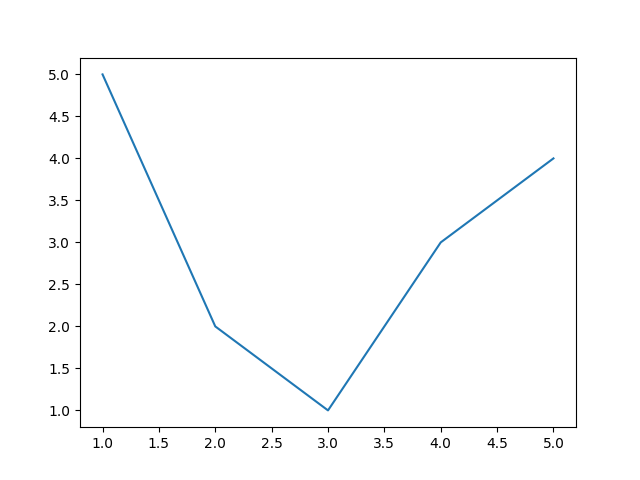
\includegraphics[scale=1.00]{images/Figure_1.png}
		\end{figure}
		
\section{Module \texttt{numpy}} \label{numpy}
	
	\subsection{Introduction au module}
		
		Le module \python|numpy| fourni non pas des fonctions, mais un nouveau type de variable~: le type \python|array|\footnote{Aussi parfois appelé "Tableau \python|numpy|"}.
		Ce type permet de construire des listes ou des tableaux de variables. Mais, contrairement aux listes Python, les \python|array| doivent respecter quelques règles~:
		\begin{itemize}
			\item la dimension est fixée lors de l'initialisation et ne peut pas être modifiée~;
			\item le type \python|array| ne peut contenir que des variables d'un seul type (e.g. on peut faire des \python|array| de \python|int|, de \python|str|, d'\python|array|, etc.).
		\end{itemize}
		En contrepartie de ces restrictions, le type \python|array| permet des manipulations plus agréables et intuitives.
		
		La dimension d'un tableau \python|numpy| est un tuple que l'on peut récupérer par la fonction~: \python|numpy.shape(mon_array)|\footnote{On pourrait également utiliser la syntaxe~: \python|mon_array.shape|.}. Si ce tuple ne contient qu'un seul nombre $n$, le tableau est unidimensionnel i.e. c'est une liste de longueur $n$~; s'il contient deux nombres $m$ et $n$, alors le tableau est bidimensionnel i.e. c'est une grille dotée de $m$ lignes et $n$ colonnes~; si la dimension est constituée de trois nombres, le tableau est dit tridimensionnel, et les trois nombres désignent sa largeur, sa hauteur et sa profondeur~; et ainsi de suite.
		
		On se contentera généralement de tableaux uni- ou bi-dimensionnels.
	
	\subsection{Tableaux \texttt{numpy}}
	
		\subsubsection{Initialisation}
		
		Il existe plusieurs méthodes d'initialisations.
		
		\subparagraph{En énumérant les éléments}
		Les tableaux \python|numpy| se comportent alors comme des listes Python, il faut donner les valeurs~: \python|numpy.array(data)|.
		Où \python|data| est une liste Python (ou un tuple). Pour un tableau bidimensionnel, \python|data| est une liste de listes de même longueur qui représentent chacune une ligne du tableau. Pour un tableau tridimensionnel, \python|data| est une liste de listes de listes, et ainsi de suite.
		
		\subparagraph{Avec la dimension}
		Si l'on connait la dimension exacte du tableau que l'on veut créer, on peut demander à \python|numpy| de construire un \python|array| de cette taille.
		Il faut alors préciser si l'on souhaite~:
		\begin{itemize}
			\item un tableau de 0~: \python|numpy.zeros(dimension)|, avec \python|dimension| la dimension du tableau souhaité, sous forme de tuple ou de liste.
			\item un tableau de nombre aléatoires~: \python|numpy.random.randint(minimum, maximum, dimension)|.
		\end{itemize}
		
		\subparagraph{Pour une courbe}
		Lorsque l'on veut calculer les points d'une courbe, on a souvent l'intervalle sur lequel il faut calculer les points et le pas\footnote{L'écart entre chaque points. Plus l'écart est grand, moins il y aura de points.}
		On utilise alors la fonction~:\\\python|numpy.arange(debut, fin, pas)|. À noter que comme pour le \python|range| du Python, la borne haute n'est pas atteinte.
		
		Dans certains cas, il est préférable de laisser \python|numpy| choisir le pas. Il faut alors lui donner un autre argument~: le nombre de points voulu.
		Il faut utiliser une autre fonction~: \python|numpy.linspace(debut, fin, nombre_points)|. Attention, ici la borne supérieure est atteinte.
	
		\subsubsection{Effets des opérateurs et fonctions}
		Les opérateurs sur les tableaux \python|numpy| ont une signification différentes de celle qu'ils ont sur les listes Python.
		
		En effet, sur les \python|array|, les opérateurs correspondent à des opérations terme à terme sur les éléments du tableau. Ainsi, additionner deux tableaux \python|numpy| revient à sommer terme à terme les éléments des tableaux. Pour avoir le droit d'effectuer une opération sur deux tableaux \python|numpy|, il faut donc que les deux tableaux soient de même dimension.
		On peut également additionner avec un scalaire pour ajouter la même valeur à toutes les cases. De même pour la soustraction, la multiplication, la division et la division euclidienne (quotient et reste).
		
		On peut également appliquer des fonctions mathématiques sur l'ensemble d'un tableau \python|numpy|.
		La syntaxe est alors plus complexe~: \python|numpy.vectorize(fonction)(tableau)|, où \python|fonction| est la fonction mathématique à appliquer sur \python|tableau|.
		
		\subsubsection{Extraction d'un sous-tableau}
		Comme pour les listes (voir~\ref{slicing}), on peut extraire un sous-tableau d'un tableau \python|numpy|, et on va là encore utiliser la syntaxe~: \python|tableau[debut: fin]|.
		La subtilité est qu'un tableau peut être $n$-dimensionnel. Il va donc falloir indiquer la zone à garder, et ce pour chaque dimension.
		
		La syntaxe est alors~: \python|tableau[debut_1: fin_1, debut_2: fin_2, ..., debut_n: fin_n]|.
		Comme pour les listes, l'indice de fin n'est jamais atteint et l'on peut utiliser des indices négatifs pour compter à partir de la fin.		
	
	\subsection{Exemples}
		
		\subsubsection{Initialisation}
		
		\begin{pythoncode}
			>>> import numpy as np
			>>> np.array([[1, 2], [3, 4]])
			array([[1, 2],
			       [3, 4]])
			>>> np.zeros((3))
			array([0., 0., 0.])
			>>> np.arange(0, 5, 0.5)
			array([0., 0.5, 1., 1.5, 2., 2.5, 3., 3.5, 4., 4.5])
		\end{pythoncode}
		
		\subsubsection{Manipulations élémentaires}
		
		\begin{pythoncode}
			>>> from math import cos
			>>> import numpy as np
			>>> tableau = np.array([[1, 2], [3, 4]])
			>>> tableau + 1
			array([[2, 3],
			       [4, 5]])
			>>> np.vectorize(cos)(tableau)
			array([[ 0.54030231, -0.41614684],
			       [-0.9899925 , -0.65364362]])
		\end{pythoncode}
		
		\subsubsection{Extraction d'un sous-tableau}
		
		\begin{pythoncode}
			>>> import numpy as np
			>>> tableau = np.array([[1, 2, 3], [4, 5, 6], [7, 8, 9]])
			>>> tableau
			array([[1, 2, 3],
			       [4, 5, 6],
			       [7, 8, 9]])
			>>> tableau[:, 0] # On ne garde que le premier élément de chaque ligne
			array([1, 4, 7])
			>>> tableau[1, 0]
			4
			>>> tableau[1:, 1:] # On garde tout à partir de la deuxième colonne et de la deuxième ligne
			array([[5, 6],
			       [8, 9]])
			>>> tableau[:2, 1:2] # On ne garde que les deux premières lignes de la deuxième colonne
			array([[2],
			       [5]])
			>>> tableau[:-1, 1:]
			array([[2, 3],
			       [5, 6]])
			>>> tableau[1:-1, 0]
			array([4])
		\end{pythoncode}
		
\section{Application}
	
	\subsection{Calcul des points d'une fonction et affichage} \label{appl:pts_fonction} (Corrigé~: \ref{corr:pts_fonction})
		
		À l'aide de deux tableaux \python|numpy|, calculez et tracez la fonction $f~:\ x \mapsto \frac{\sin(x)}{x}$. L'intervalle et le nombre de point sont laissés libre.
		Quelques grandes étapes~:
		\begin{enumerate}
			\item Choisir un intervalle sur lequel $f$ est définie et fixer un nombre de points.
			\item Commencer par créer un tableau pour les abscisses
			\item Construire le tableau pour les ordonnées
			\item Afficher le resultat
		\end{enumerate}
	
	
	
	\chapter{Gestion des fichiers}
		Ce chapitre, plutôt court, a pour but de présenter les manipulations que l'on peut faire sur des fichiers extérieurs avec Python.

\section{Ouvrir un fichier}
	
	\subsection{Chemins relatif et absolu}
		
		Pour ouvrir, lire ou écrire dans un fichier, il faut d'abord savoir où ce fichier est stocké dans la mémoire de l'ordinateur. Chaque fichier peut être trouvé dans un dossier lui-même contenu dans un dossier, et ainsi de suite, jusqu'à ce qu'on atteigne le dossier qui contient tous les autres, qu'on appelle la "racine". La suite de dossiers qui mène de cette racine à un fichier est appelée "chemin" ou "arborescence".
		
		\subsubsection{Chemin absolu}
		Le chemin absolu permet à l'ordinateur de retrouver le fichier voulu indépendemment de l'emplacement du script Python. Il donne en fait la totalité de l'arborescence du fichier depuis la racine. \\
		
		Cette méthode est pratique au sens où l'on peut changer de place le script Python sans que cela affecte son fonctionnement. Mais elle a aussi l'inconvénient de ne marcher que sur l'ordinateur sur lequel le script a été programmé. En effet le chemin absolu contient des informations propres à chaque ordinateur (notamment le nom d'utilisateur, ou le nom d'un dossier spécifique). \\
		
		Par exemple, on peut imaginer une arborescence comme celle-ci~:
		\begin{verbatim}
			/home/utilisateur/Bureau/fichier.txt
		\end{verbatim}
		Le caractère \verb|/| au début indique que l'on part de la racine de l'ordinateur, puis dans le dossier \verb|home|, puis \verb|utilisateur|, \verb|Bureau| et enfin, on s'intéresse au fichier \verb|fichier.txt|
	
		\subsubsection{Chemin relatif} \label{chemin_relatif}
		Le chemin relatif ne part pas de la racine, mais de l'emplacement du script Python. Cette méthode a l'avantage d'être adaptée au transfert d'une machine à une autre. Mais le simple fait de changer le script Python de place suffit à l'empêcher de fonctionner. \\
	
		Par exemple, nous allons créer un dossier \verb|python| sur le Bureau. Dans ce dossier, nous allons placer un script Python d'un nom quelconque ainsi qu'un dossier \verb|fichiers| qui contiendra les fichiers dont le script aura besoin. Pour l'exemple, on prendra deux fichiers~: \verb|fichier_1.txt| et \verb|fichier_2.txt|
	
		Si, depuis le script Python, on veut accéder à \verb|fichier_1.txt|, il suffira de prendre le chemin relatif~:
		\begin{verbatim}
			fichiers/fichier_1.txt
		\end{verbatim}
	
		(Un chemin relatif ne commence jamais par le symbole~: \verb|/|.) \\
		Ainsi, lors de l'utilisation de chemins relatifs, il est commode de créer un dossier avec le script Python et l'ensemble des fichiers qui sont susceptibles d'être appelés. Ainsi, changer le dossier de place n'affectera pas le fonctionnement du script.

	\subsection{Ouvrir un fichier}
	
	Pour ouvrir un fichier, nous allons faire appel à la fonction \python|open| qui va prendre deux arguments~:
	\begin{description}
		\item[le chemin] absolu ou relatif du fichier à ouvrir~;
		\item[le mode d'ouverture] un paramètre qui régit les manipulations que l'on veut effectuer sur le fichier (nous verrons ces modes plus en détatil par la suite.).
	\end{description}
	
	On a donc une syntaxe de ce type~: \python|mon_fichier = open("chemin/fichier_1.txt", "mode")|.
	Cette fonction renvoie une variable qui correspond au fichier et sur laquelle on peut effectuer des opérations (généralement lire ou écrire). Ces opérations devront néanmoins respecter le mode d'ouverture précisé lors de l'appel à la fonction.
	
	Lorsque l'on a terminé de manipuler le fichier, il est important de le fermer via la syntaxe~: \python|mon_fichier.close()|

\section{Lire un fichier}

	Il faut preciser \python|"r"| (pour "read") en mode d'ouverture du fichier, la syntaxe devient~: \python|mon_fichier = open("chemin/fichier_1.txt", "r")|.
	
	On accède ensuite au contenu lui-même via la commande~: \python|contenu = mon_fichier.read()|. Il existe deux autres fonctions qui permettent de lire dans un fichier~:
	\begin{itemize}
		\item \python|mon_fichier.readline()| qui renvoie la ligne suivante du document. (Lors du premier appel, la fonction renvoie la première ligne, puis la deuxième et ainsi de suite. Lorsqu'il n'y a plus de ligne, la fonction renvoie la chaîne vide.)
		\item \python|mon_fichier.readlines()| qui renvoie une liste qui contient toutes les lignes du document.
	\end{itemize}
	
	Et on oublie pas de fermer le fichier après. La fermeture du fichier ne modifie pas la variable \python|contenu|. On peut donc tout à fait fermer le fichier juste après avoir sauvegardé le contenu.

\section{Écrire dans un fichier}

	Il faut distinguer deux types d'écriture~:
	\begin{itemize}
		\item On ajoute du contenu à la fin du fichier, le mode d'ouverture est alors \python|"a"|, pour "append".
		\item On supprime le contenu existant et on écrit le contenu voulu dans le fichier, le mode d'ouverture est~: \python|"w"| pour "write".
	\end{itemize}
	
	Dans les deux cas, il suffit ensuite d'utiliser la commande~: \python|mon_fichier.write("...")| pour écrire dans le fichier.
	
	Notez qu'écrire dans un fichier qui n'existe pas créé le fichier.

\section{Récapitulatif}
	
	Pour manipuler des fichiers, on utilise la fonction \python|open|. Cette fonction prend en argument~:
	\begin{enumerate}
		\item le chemin (relatif ou absolu) du fichier à ouvrir~;
		\item le mode d'ouverture.
	\end{enumerate}
	
	\begin{tabular}{|c|c|} \hline
		Mode d'ouverture & Utilisation \\ \hline \hline
		\python|"r"| & lire le contenu d'un fichier \\ \hline
		\python|"w"| & écraser le contenu d'un fichier avec un nouveau contenu \\ \hline
		\python|"a"| & ajouter le nouveau contenu à la fin d'un fichier \\ \hline
	\end{tabular}

\section{Mise en pratique}
	
	\subsection{Organisation du dossier}

		Pour l'exemple, nous reprendrons la configuration prise lors de l'introduction des chemins relatifs (voir~\ref{chemin_relatif}).
		Nous allons donc prendre un dossier principal (son nom importe peu) qui va contenir~:
		\begin{enumerate}
			\item un script python (\python|test_fichier.py| dans la suite)~;
			\item un dossier du nom de \verb|fichiers| qui ne contient rien pour l'instant.
		\end{enumerate}
		
	\subsection{Écriture puis lecture d'un fichier}
		
		Le but ici est de créer un fichier contenant un texte à l'intérieur du dossier.
		Nous allons donc utiliser la commande \python|open| avec ces arguments~:
		\begin{enumerate}
			\item le chemin~: \verb|fichiers/mon_fichier.txt|
			\item le mode d'ouverture~: ici, une ouverture en écriture, donc \python|"a"| ou \python|"w"| (cela n'a pas d'importance, étant donné que le fichier n'existe pas, le contenu ne sera pas écrasé).
		\end{enumerate}

		Le code dans le fichier python va donc être~:
		\begin{pythoncode}
			mon_fichier = open("fichiers/mon_fichier.txt", "a")
			mon_fichier.write("Ceci est une phrase.")
			mon_fichier.close()
		\end{pythoncode}

		Vous pouvez ensuite ouvrir le fichier nouvellement créé avec un éditeur de texte normal pour vous assurer que l'écriture s'est bien passée. \\

		On peut également lire le contenu du fichier (attention, pour lire, il faut que le fichier existe). Le code devient alors~:
		\begin{pythoncode}
			mon_fichier = open("fichiers/mon_fichier.txt", "r")
			contenu = mon_fichier.read()
			mon_fichier.close()

			print(contenu)
		\end{pythoncode}
		
		Ce qui suit n'est pas follement intéressant c'est juste pour montrer l'utilisation de \python|readlines|.
		\begin{pythoncode}
			mon_fichier = open("fichiers/mon_fichier.txt", "a")
			mon_fichier.write("Ceci est une phrase\nEt encore une parce que sinon c'est...\npas intéressant.")
			mon_fichier.close()
			
			mon_fichier = open("fichiers/mon_fichier.txt", "r")
			print(mon_fichier.readlines())
		\end{pythoncode}

		On pourrait ensuite analyser le contenu du fichier en utilisant les manipulation vues sur les chaînes de caractères (voir~\ref{str}), la variable \python|contenu| est en effet de type \python|str|.

	
	\chapter{Algorithmes usuels et notions théoriques}
		\section{Notions préliminaires}
	
	\subsection{Invariant de boucle}
		
		On appelle "invariant de boucle" une assertion mathématique qui est vraie à chaque tour de boucle. Lors de l'exécution d'un algorithme, on peut ainsi suivre son avancement via l'invariant de boucle.
		
		Cet invariant peut servir à démontrer la correction\footnote{la correction d'un algorithme est une preuve mathématique du fait que l'algorithme fait bien ce que l'on veut.} d'un algorithme en passant par une récurrence.
	
	\subsection{Complexité d'un algorithme}
		
		La complexité est une grandeur qui caractérise le nombre de calculs que l'algorithme demande. L'avantage de cette grandeur est qu'elle est propre à l'algorithme et n'est donc pas influencée par la machine qui exécute le programme.
		
		Pour déterminer la complexité, on compte le nombre d'opérations d'un certain type, choisi de manière à avoir une grandeur pertinente. On peut, par exemple, choisir de compter les comparaisons, les multiplications, les affectations de variables etc. La complexité doit s'exprimer en fonction de la taille des données d'entrées (la longueur d'une liste, le nombre de cases d'un tableau, le nombre de chiffres d'un nombre, etc.).

	\subsection{Terminaison d'un algorithme}
		
		Vérifier la terminaison d'un algorithme, c'est vérifier qu'il ne tournera pas indéfiniment.
		
		C'est généralement assez simple à prouver. On peut décomposer les preuves de terminaison d'algorithme en trois cas~:
		\begin{itemize}
			\item Les \python|for|~: le cas le plus simple, il y a un nombre fini de tour de boucle, il reste à s'assurer qu'aucune opération illicite n'est effectuée dans la boucle (pas de division par zéro, pas d'accès à un élément d'une liste qui n'existe pas ou qui est en dehors de la liste$\ldots$)
			\item Les \python|while|~: il faut s'assurer que la condition est fausse au bout d'un nombre fini de tour, cela peut s'avérer délicat, et l'on aura souvent recourt au point suivant. Il faut également vérifier qu'aucune opération illicite n'est effectuée.
			\item Le principe de descente infinie de Fermat~: toute suite d'entier positive et strictement décroissante atteint 0 au bout d'un temps fini.
		\end{itemize}

\section{Euclide~: Calcul du plus grand diviseur commun} \label{pgcd}
	
	\subsection{Principe}
	
		L'algorithme d'Euclide permet de calculer le plus grand diviseur commun entre deux entiers. Le principe repose sur la propriété du PGCD~: $PGCD(a~;\ b) = PGCD(b~;\ r)$ en notant $r$ le reste de la division euclidienne de $a$ par $b$, de plus $PGCD(a~;\ 0) = a$. Cette propriété du PGCD consistue l'invariant de boucle.
		
		L'invariant de boucle est ici~: $PGCD(a~;\ b) = PGCD(b~;\ r)$
	
	\subsection{Terminaison}
		
		En notant $a_n$ et $b_n$ les valeurs de $a$ et $b$ au $n^{\textrm{ième}}$ tour. Au début, nous avons~: $b_0 = b$. Et à chaque tour, $b_{n + 1} = a_n \ MOD\ b_n$. Or, par définition du reste de la division euclidienne, $a \ MOD\ b < b$.
		
		Ainsi $(b_n)_{n \in \mathbb{N}}$ est une suite positive et décroissante d'entiers, donc, d'après le principe de descente infinie de Fermat~:
		\[
			\exists N \in \mathbb{N},\ b_N = 0
		\]
		D'où la terminaison de l'algorithme.
		
	\subsection{Algorithme}
		
		\begin{pythoncode}
			def pgcd(a, b):
				# tant que b est non nul
				while b != 0:
					# a prend la valeur b
					# b prend pour valeur le reste de la division euclidienne de a par b
					a, b = b, a % b
				
				# b est nul, PDCG(a, 0) = a, on renvoie donc a
				return a
		\end{pythoncode}

\section{Bézout~: résolution d'équations diophantiennes}

	\subsection{Principe}
	
		Le principe de l'algorithme de Bézout est de résoudre des équations de la forme~: $au + bv = PGCD(a~;\ b)$. Aussi appelé "algorithme d'Euclide étendu", l'algorithme de Bézout calcule le plus grand diviseur commun à $a$ et $b$, ainsi qu'une paire de coefficients $(u~;\ v) \in \mathbb{Z}^2$.
		
		L'invariant de boucle est~:
		\[ \begin{array}{rcl}
			PGCD(r1~;\ r2) & = & PGCD(a~;\ b) \\
			r1 & = & au + bv \\
			r2 & = & as + bt
		\end{array} \]
	
	\subsection{Terminaison}
	
		La terminaison est la même que pour l'algorithme d'Euclide, avec $a = r1$ et $b = r2$.
	
	\subsection{Algorithme}
	
		\begin{pythoncode}
			def bezout(a, b):
				# on initialise les variables
				u, v, s, t = 1, 0, 0, 1
				r1, r2 = a, b
				
				# tant que b est non nul
				while r2 != 0:
					# q prend pour valeur le quotient de la division euclidienne de a par b
					q = r1 // r2
					r1, u, v = = r2, s, t
					r2 = r1 % r2
					s = u - q * s
					t = v - q * t
					
				# on retourne le PGCD ainsi que les coefficients (u; v)
				return r1, u, v
		\end{pythoncode}

\section{Dichotomie}

	Les algorithmes de dichotomies sont employés pour recherher un nombre dans une liste de nombres triés. Cette méthode à l'avantage d'avoir une très bonne complexité par rapport aux algorithmes de recherche qui parcourent la liste en entier.

	\subsection{Dans une liste triée}
		
		\subsubsection{Principe}
	
		On dispose d'une liste triée \python|ma_liste|, et on sait que si l'élément \python|element| que l'on cherche est dans la liste, alors il est dans la sous-liste \python|ma_liste[mini: maxi + 1]|.
		
		Au début on pose de l'algorithme~: \python|mini = 0| et \python|maxi = len(ma_liste) - 1|. En effet, si l'élément est dans la liste, alors il est dans la sous-liste \python|ma_liste[mini: maxi + 1]| (qui correspond alors à la liste entière).
		
		Au tour suivant, on calcule l'indice central de la liste~: \python|milieu = (mini + maxi) // 2|. Or la liste est triée, donc~:
		\begin{itemize}
			\item si \python|element > ma_liste[milieu]|, alors si l'élément est dans \python|ma_liste|, il est dans la sous-liste~: \python|ma_liste[milieu + 1: maxi]|
			\item si \python|element <= ma_liste[milieu]|, alors si l'élément est dans \python|ma_liste|, il est dans la sous-liste~: \python|ma_liste[mini: milieu]|
		\end{itemize} \ \\
		
		Cet algorithme a une complexité en $\Theta (\log n)$ où $n$ est la longueur de la liste donnée en argument.
		
		\subsubsection{Terminaison}
		
		Et tant que la condition \python|mini > maxi| est vraie on tourne. À chaque tour, l'écart \python|maxi - mini|, non seulement diminue, mais est divisé par deux. Donc le programme va donc nécessairement terminer (principe de descente inifinie de Fermat). Et à la fin, si l'élément est dans \python|ma_liste|, alors \python|element = ma_liste[mini]| (ou \python|element = ma_liste[maxi]|).
		
		\subsubsection{Algorithme}
		
		\begin{pythoncode}
			def dichotomie(ma_liste, element):
				# on initialize les variables
				mini = 0
				maxi = len(ma_liste) - 1
				
				while mini > maxi:
					# on calcule l'indice du milieu de la sous-liste
					milieu = (mini + maxi) // 2
					
					# on regarde dans quelle moitié de la sous-liste l'élément peut être
					if element > ma_liste[milieu]:
						mini = milieu + 1
					else:
						maxi = milieu
				
				return element == ma_liste[mini]
		\end{pythoncode}
	
	\subsection{Sur une fonction monotone}
		
		\subsubsection{Principe}
		
		De manière analogue à la précédente~; on cherche à trouver le point d'annulation d'une fonction monotone sur un intervalle $[mini~;\ maxi]$ avec une certaine précision.
		
		Comme pour la première version, on va calculer le milieu de l'intervalle et distinguer deux cas~:
		\begin{itemize}
			\item si $f(mini) \cdot f(milieu) > 0$~: $f(mini)$ et $f(milieu)$ sont donc de même signe or la fonction est monotone, donc le point d'annulation est après le milieu de l'intervale
			\item sinon, le points d'annulation est avant le milieu de l'intervalle
		\end{itemize} \ \\
		
		En comptant le nombre de tour de boucle, la complexité est un $\Theta (n)$ où $n$ est la précision (en bit) du résultat. Autrement dit, plus le résultat est précis, plus l'éxecution du programme sera longue.
		
		\subsubsection{Terminaison}
		
		En notant $a_n$ et $b_n$ les valeurs de $a$ et $b$ au $n^{\textrm{ième}}$ tour. Au sein d'un tour de boucle, on a~:
		\[
			\forall n \in \mathbb{N}^*,\ b_{n+1} - a_{n+1} = \frac{b_n - a_n}{2}
		\]
		
		Par récurrence, au bout de $k$ tours de boucle~:
		\[
			0 < b_k - a_k = \frac{b - a}{2^k}
		\]
		
		Or, $\frac{b - a}{2^k} \underset{k \to +\infty}{\longrightarrow} 0$ ainsi~:
		\[
			\forall \varepsilon > 0,\ \exists N \in \mathbb{N}^*,\ |b_N - a_N| < 2 \varepsilon
		\]
		
		\subsubsection{Algorithme}
			
		\begin{pythoncode}
			def dichotomie(f, mini, maxi, precision):
				while (maxi - mini) > 2 * precision:
					milieu = (maxi - mini) / 2
					if f(mini) * f(milieu) > 0:
						mini = milieu
					else:
						maxi = milieu
				return (maxi - mini) / 2
		\end{pythoncode}

\section{Méthode des rectangles et des trapèzes~: approximation d'une intégrale}
	
	\subsection{Principe}
		
		On considére une subdivision de l'intervalle sur lequel on veut approximer l'intégrale de $f$. Et pour chaque petit intervalle on va approximer la fonction par une fonction constante, ainsi, calculer l'aire sous la courbe va revenir à un calcul d'aire de rectangle (voir Figure~\ref{fig_3}).
		
		 On se place ainsi sur un segment $[a~;\ b]$ et on fixe un nombre arbitraire $n$ de subdivisions sur ce segment. Les largeurs des subdivisions sont égales\footnote{On parle alors de subdivision à pas constant.}, et valent~: $\frac{b - a}{n}$.
		 
		 La fonction étant approximée par une fonction constante, la hauteur du $k^{\textrm{ième}}$ rectangle vaut $f(a + k * largeur)$. Ainsi l'aire sous le $k^{\textrm{ième}}$ rectangle est de~: $\frac{b - a}{2} \cdot f \left( a + k \cdot \left( \frac{b - a}{2} \right) \right)$
		
		\begin{figure}[H]
			\centering
			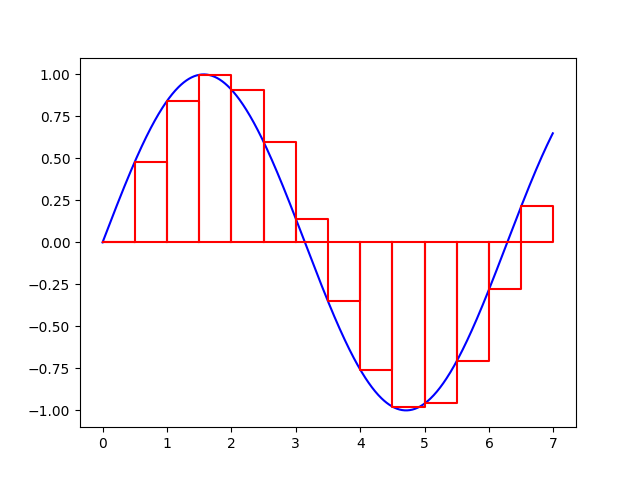
\includegraphics[scale=0.75]{images/Figure_3.png}
			\caption{Approximation de la fonction $sin$ avec un pas de 0.5}
			\label{fig_3}
		\end{figure}
	
	\subsection{Terminaison}
		
		Montrer la terminaison ne pose pas de problème~: l'algorithme repose sur une boucle itérative finie et aucune opération illicite n'est effectuée.
	
	\subsection{Algorithme}
	
		\begin{pythoncode}
			def rectangle(f, a, b, n):
				# l'aire vaut zéro au début
				integrale = 0
				
				# le pas étant constant, la largeur est la même partout
				largeur = (b - a) / n
				
				for k in range(n):
					# on calcule la hauteur
					hauteur = f(a + k * largeur)
					
					# on ajoute l'aire du rectangle à l'intérgrale
					integrale += hauteur * largeur
				
				# on renvoie la somme des aires des rectangles
				return integrale	
		\end{pythoncode}
	
	\subsection{Méthode des trapèzes}
		
		La méthode est sensiblement la même, mais on approxime la fonction par des fonctions affines et non plus des constantes.
		
		\begin{figure}[htp]
			\centering
			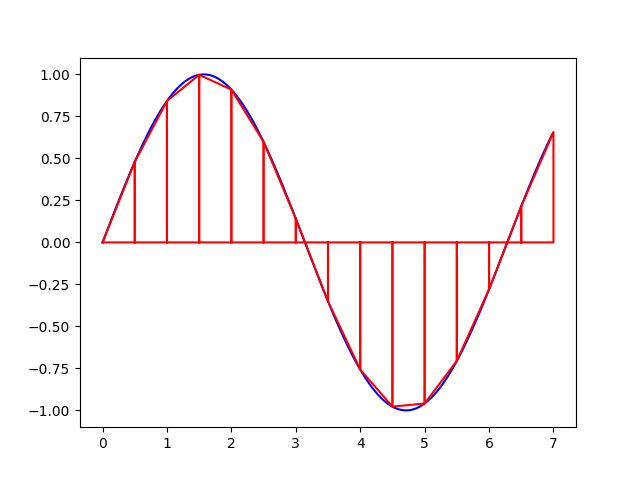
\includegraphics[scale=0.75]{images/Figure_4.png}
			\caption{Approximation de la fonction $sin$ avec un pas de 0.5}
		\end{figure}
		
		La largeur ne change pas par rapport à la méthode des rectangles, mais la hauteur devient la moyenne entre $f(a + k * largeur)$ et $f(a + (k + 1) * largeur)$. Ainsi~:
		
		\begin{pythoncode}
			def trapeze(f, a, b, n):
				integrale = 0
				largeur = (b - a) / n
				
				for k in range(n):
					hauteur = f(a + k * largeur) + f(a + (k+1) * largeur)
					integrale += largeur * hauteur / 2
				
				return integrale
		\end{pythoncode}

\section{Méthode d'Euler~: résolution d'une équation différentielle}
	
	\subsection{Principe}
		
		Cette méthode permet de résoudre des équations différentielles d'ordre 1 de la forme~:
		\[
			\forall t \in [a~;\ b],\ y'(t) = f(t, y(t))
		\]
		dans lesquelles on cherche $y$.
		
		On considère les conditions initiales~: $(t_0~;\ y_0)$ telles que $y_0 = y(t_0)$, et un intervalle $[0~;\ T]$ dans lequel va varier $t$. L'enjeu est de prendre des valeurs suffisamment proches tout en conservant un temps de calcul raisonnable, à l'instar de la méthode des rectangles, nous allons subdiviser l'intervalle $[a~;\ b]$ en $N$ sous-intervalles de longeur~: $h = \frac{b - a}{N}$\footnote{$h$ est le pas et l'on a~: $t_{n+1} = t_n + h$}. On définit alors les valeurs de $t_n$ pour lesquelles on va approximer $y(t_n)$ par $y_n$~:
		\[
			\forall n \in \llbracket 0~;\ N \rrbracket,\ t_n = nh
		\]
		
		Ainsi, nous allons avoir une suite $(y_n)_{n \in \llbracket 0~;\ N \rrbracket}$ et~:
		\[
			 \forall n \in \llbracket 0~;\ N \rrbracket,\ y_n \approx y(t_n)
		\]
		
		Les $y_n$ sont calculables de proche en proche grâce à la formule de récurrence~:
		\[
			\forall n \in \llbracket 0~;\ N \rrbracket,\ y_{n+1} = y_n + h \cdot f(t, y_n)
		\]
		
		Il restera enfin à tracer la courbe des $y_n$ (voir chapitre~\ref{chap_4}).
	
	\subsection{Terminaison}
		
		Comme pour la méthode des rectangles, il n'y a qu'une boucle for, ni aucune opération illicite, donc le programme termine.
		
	\subsection{Algorithme}
		
		Avec des listes Python~:
		\begin{pythoncode}
			def euler(f, a, b, N, y0):
				# on calcule le pas
				h = (b - a) / N
				
				# construction des abscisses
				X = [a + n * h for n in range(N)]
				
				# on simplifie un peu le problème en considérant y(a) = y0
				Y = [y0]
				
				# N - 1 car la première valeur (condition initiale) est déjà dans la liste
				for i in range(N - 1):
					# on extrait le tn et yn
					t, y = X[i], Y[i]
					
					# calcul de y_{n+1}
					y = y + h * f(t, y)
					
					# on stocke la nouvelle valeur de y (y_{n+1})
					Y.append(y)
				
				# on renvoie les points calculés (pour tracer une courbe par exemple)
				return X, Y
		\end{pythoncode}
		On peut tout à fait raccourcir la boucle \python|for| en~:
		\begin{pythoncode}
			for i in range(N - 1):
				Y.append(Y[i] + h * f(X[i], Y[i]))
		\end{pythoncode}
		
		Avec des \python|array| (voir~\ref{numpy})~:
		\begin{pythoncode}
			def euler(f, a, b, N, y0):		
				X = np.linspace(a, b, N)
				Y = np.zeros(N)
				
				# condition initiale y(a) = y0
				Y[0] = y0
				
				# calcul du pas
				h = (b - a) / N
				
				# calcul des abcisses
				for i in range(N):
					Y[i + 1] = Y[i] + h * f(X[i], Y[i])
				
				return X, Y
		\end{pythoncode}
	
	\subsection{Application} \label{appl:equa_diff} (Corrigé~: \ref{corr:equa_diff})
		
		On cherche à résoudre l'équation différentielle~:
		\[
			\forall t \in [-1~;\ 10],\ (t^2 + 1)y' + (t - 1)^2y = t^3 - t^2 + t + 1
		\]
		Avec la condition initiale~: $y(-1) = 8$.
		Le but est de reprogrammer l'algorithme, pas d'utiliser les fonctions.
		
		Les grandes étapes~:
		\begin{enumerate}
			\item Il faut commencer par isoler $y'$ pour trouver $f$, une fonction de $t$ et de $y$.
			\item Construire le tableau des ordonnées.
			\item Construire les abcisses de la solution pour une condition initiale donnée.
			\item Tracer la courbe de la solution.
			\item (Juste parce que c'est joli, recommencer avec une autre condition initiale.)
		\end{enumerate}

\section{Exponentiation rapide}
	
	\subsection{Principe}
		
		Dans toute cette sous-section, nous voulons élever $x \in \mathbb{R}$ à une puissance $p \in \mathbb{N}^*$. Partons de l'algorithme naïf, récursif d'exponentiation~:
		\begin{pythoncode}
			def puissance(x, p):
				if p == 0: return 1
				else: return x * puissance(x, p - 1)
		\end{pythoncode}
		
		Ainsi, cet algorithme va effectuer $p$ tours de boucles avant de terminer. Sa complexité est donc un $\Theta(p)$. Cette complexité n'est pas catastrophique, mais on peut mieux faire. Pour cela il faut remarquer trois choses~:
		\begin{itemize}
			\item si $p = 0$, $x^p = 1$
			\item si $p$ est pair, $x^p = (x^2)^{\frac{p}{2}}$
			\item si $p$ est impair, $x^p = x \times (x^2)^{\frac{p - 1}{2}}$
		\end{itemize}
		
		Ainsi, si $p$ est pair, on peut calculer $y^{\frac{p}{2}}$ avec $y = x^2$, si $p$ est impair, on calcule $y^{\frac{p - 1}{2}}$ avec $y = x^2$ et on multiplie par $x$.
		
		La différence peut sembler futile, mais si on représente le nombre de multiplication effectuées pour calculer les puissances de 5 de 1 à 100~:
		\begin{figure}[htp]
			\centering
			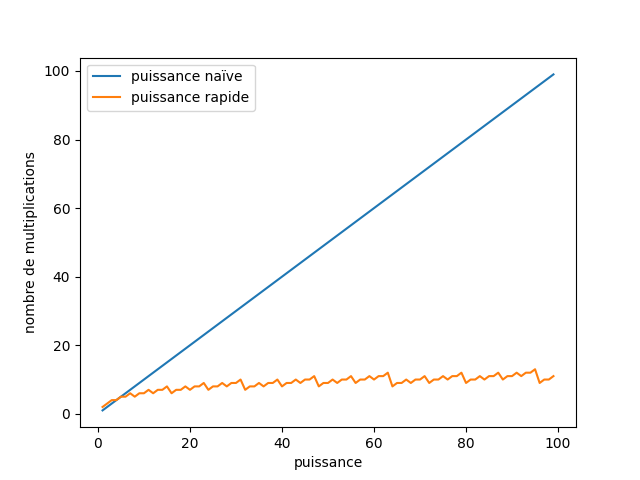
\includegraphics[scale=0.75]{images/Figure_7.png}
			\caption{Nombre de multiplications effectuées en fonctions de la puissance}
		\end{figure}
		On se rend compte que l'algorithme rapide est réellement plus performant que l'algorithme naïf. De plus, on peut montrer par le calcul que l'exponentiation rapide a une complexité en $\Theta (\log n)$.
		
	\subsection{Terminaison}
		
		L'algorithme termine car $p$ est un entier postif, qui décroît à chaque tour de boucle (il est divisé par deux à chaque fois). Donc d'après le principe de descente infinie de Fermat, $p$ va finir par être nul.
	
	\subsection{Algorithme}
		On peut écrire une version récursive~:
		\begin{pythoncode}
			def puissance_rapide(x, p):
				if p == 0: return 1
				elif p % 2: return x * puissance(x**2, (p - 1) // 2) # si p % 2 != 0 donc si p est impair
				else: return puissance(x**2, p // 2)
		\end{pythoncode}


\section{Binaire et changement de bases}

	\subsection{Principe}
		
		Dans les ordinateurs, les nombres sont représentés par une représentation dite en "binaire". Il s'agit d'une succession de 0 et de 1 qui correspondent au nombre. De manière courante nous utilisons la notation en base 10. L'enjeux de cette partie est de voir comment baser du binaire au décimal et d'implémenter cet algorithme. Dans la représentation binaire, on appelle nombre de bits le nombre de chiffres. Quelques exemples sur deux bits~: \\
		\begin{tabular}{|l|l|} \hline
			décimal & binaire \\ \hline
			0 & 00 \\ \hline
			1 & 01 \\ \hline
			2 & 10 \\ \hline
			3 & 11 \\ \hline
		\end{tabular} \\

		Pour passer du binaire au décimal, il faut écrire chaque chiffre du nombre ainsi que la puissance de 2 auquel il est associé. La méthode générale est de partir du chiffre le plus à gauche et de lui associé la puissance $2^0$, le chiffre juste à droite reçoit reçoit la puissance $2^1$ et ainsi de suite. Par exemple, si l'on prend le nombre écrit en binaire $1011$~:
		\[ \begin{array}{llll}
			2^3 & 2^2 & 2^1 & 2^0 \\
			1   & 0   & 1   & 1 \\
		\end{array} \]
		
		Ainsi $1011$ en binaire, peut se décomposer en décimal comme $1 \times 2^3 + 0 \times 2^2 + 1 \times 2^1 + 1 \times 2^0$, d'où~:
		\[ \begin{array}{rcl}
			1 \times 2^3 + 0 \times 2^2 + 1 \times 2^1 + 1 \times 2^0 & = & 1 \times 8 + 0 \times 4 + 1 \times 2 + 1 \times 1 \\
			& = & 8 + 2 + 1 \\
			& = & 11
		\end{array} \]
		Ainsi le nombre $1011$ en binaire est équivalent au nombre $11$ en décimal. \\
		
		Pour passer du décimal au binaire, il faut décomposer le nombre en décimal en effectuant des disivions euclidiennes par deux et en gardant les restes tant que le quotient est non nul. Reprenons $11$ comme point de départ.
		\begin{itemize}
			\item on divise $11$ par $2$. $11 = 2 \times 5 + 1$, on garde le $1$
			\item $5 = 2 \times 2 + 1$, on place ce deuxième reste ($1$) à droite du premier. (le nombre décomposé en binaire ressemble alors à~: $..11$).
			\item $2 = 2 \times 1 + 0$ donc on met le $0$ à droite des deux premiers chiffres et on continue car $1$ est non nul
			\item $1 = 2 \times 0 + 1$ on place alors ce dernier reste à droite des trois premiers chiffres et on s'arrête car le quotient est nul.
		\end{itemize}
		
		On retrouve alors le nombre $1011$ en binaire.

	\subsection{Terminaison}
		
		Dans le cas du passage du binaire vers le décimal, l'algorithme va devoir parcourir tous les chiffres du nombre, la boucle \python|for| ne contenant pas d'opérations illicites, l'algorithme est fini.
		
		Pour le cas de la conversion, l'algorithme boucle tant que le quotient est non nul, or le quotient est divisé par deux au tour suivant. Ainsi la suite des quotients au fil des tours de boucle forme une suite d'entiers positifs décroissantes, donc il existe un quotient nul, d'où la terminaison de l'algorithme.
	
	\subsection{Algorithme}
		
		Pour passer du binaire au décimale, la fonction va prendre en argument le nombre au format binaire dans une chaîne de caractère et appliquer le principe vu plus haut, de manière à renvoyer un entier en base 10.
		\begin{pythoncode}
			def decimal(nb_binaire):
				resultat = 0
				for i in range(len(nb_binaire)):
					chiffre = int(nb_binaire[-(i + 1)] # on extrait le chiffre d'indice i en partant de la fin
					puissance_deux = 2 ** i # on calcule la puissance de 2 correspondante
					resultat += chiffre * puissance_deux # on ajoute au résultat
				return resultat
		\end{pythoncode}
		
		Pour convertir un nombre du format décimal vers le binaire, nous allons faire une fonction qui va prendre en argument le nombre à convertir et qui va renvoyer la liste des chiffres en binaire.
		\begin{pythoncode}
			def binaire(nb_decimal):
				resultat = [nb_decimal % 2] # on initialise la liste avec le premier reste
				nb_decimal //= 2 # on divise le nombre pour garder le quotient
				while nb_decimal: # tant que le quotient est non nul
					resultat.insert(0, nb_decimal % 2) # on insert à droite du premier élément, le reste suivant
					nb_decimal //= 2 # on calcule le quotient suivant
				return resultat # on renvoie la liste des restes
		\end{pythoncode}

\section{Tri par insertion}
	
	\subsection{Principe}
		
		Le principe est de parcourir la liste, et tant que l'élément que l'on regarde est plus petit que l'élément précédent et que les indices sont positifs, on inverse les éléments.\\
		
		En prenant $n$, la longueur de la liste, la complexité est en $\Theta(n)$ si la liste est déjà triée (complexité dans le meilleur cas), et peut atteindre $\Theta(n^2)$ dans le pire cas.
		
	\subsection{Terminaison}
		
		La boucle \python|while| termine car soit l'élément que l'on déplace est décalé jusqu'à la première case de la liste, soit l'élément se retrouve à sa place. La boucle \python|for| termine car on ne parcourt la liste qu'une seule fois.
	
	\subsection{Algorithme}

		\begin{pythoncode}
			def tri_insertion(liste):
				for i in range(1, len(liste)):
					element_a_trier = liste[i]
					j = i
					while j > 0 and element_a_trier < liste[j - 1]: # tant que 'element_a_trier' n'est pas à sa place et que l'indice est positif
						liste[j] = liste[j - 1] # on recule l'élément à trier dans la liste
						j -= 1 # on recule l'indice de l'élément comparé
					liste[j] = element_a_trier # on insert l'élément à trier à sa place
		\end{pythoncode}
		
\section{Tri-fusion}
	
	\subsection{Principe}
		
		Le tri fusion repose sur un principe simple~:
		\begin{itemize}
			\item une liste a un seul élément est triée
			\item pour trier une liste à $n$ éléments on fusionne les deux sous-listes de longeurs égales extraites de cette liste
		\end{itemize}
		
		On va donc commencer par diviser la liste donnée en argument en plusieurs sous-listes jusqu'à obtenir des listes de longueur 1. On triera ensuite les listes en les fusionnant. \\
		
		Le fonctionnement de la fusion est central. On note $a$ et $b$ les deux sous-listes à fusionner et $a_i$ et $b_i$ les $i^{\textrm{ième}}$ éléments des listes $a$ et $b$. On prend un indice $i$ associé à la liste $a$ et un indice $j$ associé à $b$. 
		
		On initialise $i$ et $j$ à $0$, et on créée une liste vide $c$ munie d'un indice $k$ initialisé à $0$ aussi.
		
		Tant que $i$ est inférieur à la taille de $a$ et $j$ est inférieur à la taille de $b$, on boucle suivant le principe suivant~:
		\begin{itemize}
			\item si $a_i \leq b_j$, on ajoute $a_i$ à $c$, on incrémente $i$ de un
			\item si $a_i > b_k$, on ajoute $b_j$ à la liste $c$, et on incrémente $j$ de un
		\end{itemize}
		La liste $c$ est alors la liste triée résultant de la fusion entre $a$ et $b$. \\
		
		La complexité du tri-fusion dans le pire cas se divise en trois parties~: le tri de la première sous-liste, de la seconde sous-liste, et la fusion des deux. On peut alors montrer que si la liste donnée est de taille $n$ la complexité est en $\Theta(n \log n)$.
		
	\subsection{Terminaison}
	
		L'algorithme de fusion est terminé, puisqu'à chaque tour, soit $i$ soit $j$ augmente d'un, donc on finit par atteindre la taille des sous-listes.
		e
		La fonction principale va découper la liste en sous-liste de longeur $\frac{n}{2}$ à chaque tour, donc on finira par avoir des listes de longueurs un qui sont, par définition, déjà triées.
		
	\subsection{Algorithme}
		
		\begin{pythoncode}
			def fusion(a, b):
				i = j = 0
				c = []
				while i < len(a) or j < len(j):
					if j == len(b) or (i < len(a) and a[i] <= b[j]):
						c.append(a[i])
						i += 1
					elif i == len(a) or (j < len(b) and a[i] > b[j]):
						c.append(b[j])
						j += 1
				return c
			
			def tri_fusion(liste):
				n = len(liste)
				if n == 1: return liste
				else: return fusion(tri(liste[n // 2: ]), tri(liste[: n // 2]))
		\end{pythoncode}
			
			
				

	
	\chapter{Programmation orientée objet}
		\section{Introduction à la programmation orientée objet (POO)}

	\subsection{Définition d'un objet et principe de la POO}
	
		En Python, toutes les variables sont typées (i.e. ont un type). Ainsi lorsque l'on écrit~: \python|variable = 4|, on crée en fait un objet \python|variable|, de type \python|int| et qui contient \python|4| (la valeur elle-même a aussi le statut d'objet).
		
		On dit que \python|variable| est une instance du type \python|int|. Ce qui explique pourquoi \python|4| a également le statut d'objet~: il s'agit bien d'une instance aussi.
		
		De manière un peu plus formelle, une instance est un représentant d'un type donné. Le type est une notion abstraite (un entier, une liste etc) alors que l'instance est un objet particulier rattaché à cette notion (\python|4| est un entier en particulier, et non un entier en tant que notion).
			
		La programmation orientée objet va avoir pour objectif de créer de nouveaux types de variables. On pourra ensuite écrire \python|ma_variable = MonType()| où \python|ma_variable| sera une instance (un objet) du type \python|MonType|.
	
	\subsection{Classes, méthodes et attributs}
		
		\subsubsection{Première approche pratique}
		Reprenons un exemple~: \python|ma_liste = [1, 2, 3]|. Ici, \python|ma_liste| est une instance du type \python|list|. On dit qu'on accède à une méthode ou à un attribut d'une instance lorsqu'on utilise la syntaxe avec le point~: \python|mon_instance.methode()|, ou \python|mon_instance.attribut|.
		
		Sur les listes par exemple, lorsque l'on écrit~: \python|ma_liste.append(2)|, on appelle en fait la méthode \python|append| associée au type \python|list| (toutes les listes ont cette méthode), avec l'argument \python|3|. Les méthodes sont de ce fait des fonctions associées à un type précis.
		
		Les attributs correspondent à des variables propre à un type. Il y a assez peu d'exemple en Python, on pourra toutefois citer les tableaux \python|numpy| qui ont un attribut \python|shape| qui correspond à la taille du tableau.
		
		\subsection{Formalisation}
		En résumé~:
		\begin{description}
			\item[Une méthode] est une fonction associée à un type précis.
			\item[Un attribut] est une variable associée à un type précis.
		\end{description}
		Et on appelle une méthode (ou on demande la valeur d'un attribut) grâce au point que l'on place entre l'instance et la méthode (ou l'attribut).
		
		Donc pour l'instant, on a vu qu'un type est en fait constitué de fonctions (méthodes) et de variables (attributs). Pour programmer un nouveau type, il faut indiquer explicitement à Python quelle fonction (ou variable) est une méthode (ou attribut) du nouveau type. Pour cela on utilise une classe. La syntaxe est assez simple~:
		\begin{pythoncode}
			class MonType:
				attribut = <valeur>
				def methode(<argument>):
					<actions>
					return <variable>
		\end{pythoncode}

\section{Classes et types}
	
	\subsection{Créer un nouveau type}
		
		Créer un nouveau type de variable est équivalent à créer une classe. Il suffit dont d'écrire~: 
		\begin{pythoncode}
			class MonType:
				pass
		\end{pythoncode}
		Le mot-clef \python|pass| permet de dire à Python qu'il n'y a rien à faire.\footnote{i.e. que la classe est vide, que la fonction n'effectue aucun calcul etc.} Dans la suite nous verrons comment remplir cette classe avec des méthodes et des attibuts.
		
		On peut ensuite écrire~: \python|ma_variable = MonType()| pour créer une instance du type \python|MonType|.
	
	\subsection{Implémentation de méthodes et d'attributs}
	
		Pour définir une nouvelle méthode, il suffit d'écrire une fonction dans la classe. Cette fonction peut prendre des arguments et renvoyer (ou afficher) un résultat, comme n'importe quelle fonction.
		
		La seule subtilité est que toutes les méthodes doivent prendre au moins un argument~: l'instance elle-même. Explications~: lorsque l'on écrit~: \python|ma_variable = MonType()|, on crée une instance qui porte le nom \python|ma_variable|. Les méthodes vont donc prendre cette instance en premier argument, qui est nommé \python|self| par convention.
		
		Si l'on reprend notre exemple~:
		\begin{pythoncode}
			class MonType:
				def methode(self):
					return 42
		\end{pythoncode}
		
		On peut ensuite créer une instance pour voir le résultat (limité pour l'instant)~:
		\begin{pythoncode}
			>>> variable = MonType()
			>>> variable.methode()
			42
		\end{pythoncode}
		
		Pour créer un attribut, ce n'est pas plus compliqué qu'une simple affectation.
		\begin{pythoncode}
			class MonType:
				def methode(self):
					self.attribut = 0
					return 42
		\end{pythoncode}
		
		Bien que ce code soit fonctionnel, nous rencontrons quelques paradoxes~: l'attribut est défini à l'intérieur d'une méthode, si bien que tant que cette méthode n'a pas été exécutée, l'attribut n'existe pas. Ainsi~:
		\begin{pythoncode}
			>>> variable = MonType()
			>>> variable.attribut
			AttributeError
			>>> variable.methode()
			42
			>>> variable.attribut
			0
		\end{pythoncode}
		
		On voudrait pourtant pouvoir utiliser l'attribut comme une propriété de l'instance indépendamment des méthodes exécutées. La méthode spéciale \python|__init__| permet de pallier ces problèmes de définition.
	
	\subsection{Méthodes spéciales}
		
		Python permet de nombreuses manipulations avec les objets comme la re-définition des opérateurs pour le nouveau type (\python|+|, \python|-|, \python|*|, \python|/|, ...), mais aussi la possibilité de rendre l'objet "appelable", ou "itérable". Ces notions seronts vues en même temps que les méthodes spéciales correspondantes.
		
		Avant de voir ces méthodes spéciales, un petit point de syntaxe, dans une classe, les méthodes spéciales sont toujours de la forme \python|__methode__(self, <argument>):|.
		
		\subsubsection{Initialiser un objet}
		La méthode spéciale \python|__init__| se lance automatiquement à la création de l'instance. Ainsi, lorsque l'on écrit~: \python|variable = MonType()|, la méthode \python|__init__| se lance. 
		
		Il faut voir la création de l'instance comme un appel à \python|__init__|, le premier argument est l'instance elle-même (\python|self| par convention), les arguments suivants sont des arguments normaux. Par exemple, si l'on définit la classe par~:
		\begin{pythoncode}
			class MonType:
				def __init__(self, attribut):
					self.attribut = attribut
		\end{pythoncode}
		On peut ensuite s'en servir de la manière suivante~:
		\begin{pythoncode}
			>>> variable = MonType(1)
			>>> variable.attribut
			1
		\end{pythoncode}
		
		Contrairement à l'attribut défini dans l'exemple du paragraphe précédent, cet attribut pourra être utilisé dans toutes les méthodes de la classe sans problème.
		
		\subsubsection{Redéfinition des opérateurs}
		Nous ne verrons ici que comment redéfinir les opérateurs élémentaires, à savoir l'addition, la soustraction, la multiplication et la division.
		
		Un peu de théorie avant la suite, lorsque l'on écrit un calcul, Python lance en fait une méthode qui correspond au calcul à effectuer. Ainsi \python|2+3| exécute une méthode sur les \python|int|, \python|"bon" + "jour"| lance la même méthode, mais sur les \python|str|. \\
		
		Un peu plus de subtilité, pour chaque opérateur, il existe deux méthodes qui correspondent aux deux syntaxes~:
		\begin{itemize}
			\item \python|variable <operateur> <argument>| qui est la syntaxe normale, avec l'instance à gauche.
			\item \python|<argument> <operateur> variable| qui est la syntaxe inverse avec l'instance à droite.
		\end{itemize}
		
		La liste des principaux opérateurs~:
		\begin{itemize}
			\item L'addition correspond à la méthode spéciale~: \python|__add__(self, argument):|. Cette méthode est appelée avec la syntaxe~: \python|variable + <argument>|. Dans les faits, la commande~: \python|a = b + c| devient~: \python|a = b.__add__(c)|\footnote{Le principe est le même pour les autres opérateurs}.
			\item La soustraction peut-être implémentée avec la méthode \python|__sub__(self, argument):|.
			\item La multipliciation par \python|__mul__(self, argument):|.
			\item Et la division par \python|__truediv__(self, argument):|.
		\end{itemize}
		
		Les méthodes sont les syntaxes inverses ont les même noms précédés d'un "r". Ainsi, la syntaxe inverse pour l'addition correspond à la méthode spéciale~: \python|__radd__(self, argument):|.
		
		En général, les opérateurs sont symétriques, on peut donc définir les méthodes des syntaxes inverses par la syntaxe~: \python|__roperateur__ = __operateur__|.
		
		Par exemple~:
		\begin{pythoncode}
			class MonType:
				def __init__(self, attribut):
					self.attribut = attribut
				
				def __add_(self, nombre):
					return self.attribut + nombre
				
				def __radd_(self, nombre):
					return self.attribut * nombre
		\end{pythoncode}
		Et en pratique~:
		\begin{pythoncode}
			>>> variable = MonType(2)
			>>> variable + 5 # __add__
			7
			>>> 2 + variable # __radd__
			10
		\end{pythoncode}
		
		\subsubsection{Appeler une instance de la classe}
		Lorsque l'on appelle une fonction, on utilise une syntaxe avec des parenthèses. L'idée est la même ici, on va rendre les instances de notre classe "appelables" ainsi, lorsque l'on écrira~: \python|variable(<arguments>)|, Python exécutera une méthode avec les arguments donnés.
		
		La méthode en question est~: \python|__call__(self, <arguments>):|. Un petit exemple pour comprendre~:
		\begin{pythoncode}
			class MonType:
				def __init__(self, attribut):
					self.attribut = attribut
				
				def __call__(self, nombre):
					return self.attribut * nombre
		\end{pythoncode}
		Et l'exécution~:
		\begin{pythoncode}
			>>> variable = MonType(2)
			>>> variable(5) # 2 * 5
			10
		\end{pythoncode}
		
		\subsubsection{Rendre une classe indexable}
		Un exemple connu d'objet indexable sont les listes, ou les chaînes de caractères. Plus généralement les instances de la classe vont réagir à la syntaxe~: \python|variable[<arguments>]|. On peut mettre à peu près tout et n'importe quoi dans les crochets.
		
		La méthode spéciale est ici~: \python|__getitem__(self, arguments):|. Comme tout à l'heure, un exemple~:
		\begin{pythoncode}
			class MonType:
				def __init__(self, attribut):
					self.attribut = attribut
				
				def __getitem__(self, nb):
					return self.attribut * nb
		\end{pythoncode}
		Et avec un exemple d'utilisation~:
		\begin{pythoncode}
			>>> variable = MonType(5)
			>>> variable[2]
			10
		\end{pythoncode}
		
		\subsubsection{Afficher un objet}
		Il y a deux manière d'afficher un objet~:
		\begin{itemize}
			\item En programmant le transtypage vers le type \python|str| via la méthode spéciale~: \python|__str__(self)|, on affiche alors via la fonction \python|print|.
			\item En programmant la représentation de l'objet via~: \python|__repr__(self)|, l'affichage se fait alors par un simple appel à la variable.
		\end{itemize}
		
		Dans les deux cas, la fonction va devoir renvoyer la chaîne de caractères.
		
		Premier exemple avec le transtypage~:
		\begin{pythoncode}
			class MonType:
				def __init__(self, attribut):
					self.attribut = attribut
				
				def __str__(self):
					return str(self.attribut) # on renvoie la représentation sous forme de chaîne de caractères
		\end{pythoncode}
		En pratique~:
		\begin{pythoncode}
			>>> variable = MonType(2)
			>>> print(variable)
			2
		\end{pythoncode}
		
		Second exemple avec la représentation~:
		\begin{pythoncode}
			class MonType:
				def __init__(self, attribut):
					self.attribut = attribut
				
				def __repr__(self):
					return str(self.attribut)
		\end{pythoncode}
		Et~:
		\begin{pythoncode}
			>>> variable = MonType(2)
			>>> variable
			2
		\end{pythoncode}
		
		\subsubsection{Récapitulatif}
			
		\begin{tabular}{|c|c|} \hline
			Méthode spéciale & Effet \\ \hline \hline
			\python|__init__| & Initialiser l'objet \\ \hline
			\python|__add__| & Addition \\ \hline
			\python|__sub__| & Soustraction \\ \hline
			\python|__mul__| & Multiplication \\ \hline
			\python|__truediv__| & Division \\ \hline
			\python|__call__| & Rendre une classe appelable \\ \hline
			\python|__getitem__| & Rendre une classe indexable\\ \hline
			\python|__str__| et \python|__repr__| & Afficher un objet \\ \hline
		\end{tabular}
	
	\subsection{Héritages}
		
		En Python, et dans les autres langages orientés objets aussi, une classe peut hériter des méthodes et attributs d'une autre classe. Ainsi, la nouvelle classe contiendra toute les méthodes de la classe dont elle a héritée plus de nouvelles méthode (ou attributs) qui seront rajoutés "par dessus" la classe d'origine.
		
		Pour faire en sorte qu'une classe \python|ClassA| hérite d'une classe \python|ClassB|, on écrit~: \python|class ClassA(ClassB)|.
		
		Ici, nous allons nous intéresser à un exemple un peu plus concret que ceux vu plus haut dans ce chapitre~: nous allons créer un nouveau type de chaînes de caractères, basé sur les \python|str|. Nous allons donc commencer par~:
		\begin{pythoncode}
			class Str(str): # Python est sensible à la casse, donc pas de risque
				def __init__(self, valeur):
					self.data = valeur
				
				def methode(self):
					return 42
		\end{pythoncode}
		Ici, les instances de classe \python|Str| vont se comporter exactement comme des chaînes de caractères normale, mais on peut leur appliquer la méthode \python|methode()| qui renvoie 42.
		\begin{pythoncode}
			>>> variable = Str("Ceci est une chaîne")
			>>> variable.methode()
			42
		\end{pythoncode}
		
		On peut également s'amuser à redéfinir les opérateurs sur les entiers~:
		\begin{pythoncode}
			class Int(int):
				def __init__(self, valeur):
					self.valeur = valeur
				
				def __add__(self, b):
					return self.valeur * b
				
				def __sub__(self, b):
					return self.valeur + b
				
				def __mul__(self, b):
					return self.valeur / b
				
				def __truediv__(self, b):
					return self.valeur - b
		\end{pythoncode}
		Et pour montrer les effets~:
		\begin{pythoncode}
			>>> var_a = Int(2)
			>>> var_b = Int(5)
			>>> var_a + var_b
			10
			>>> var_a # __repr__ n'est pas programmée, mais l'héritage fait que la méthode fonctionne
			2
			>>> var_a / var_b
			7
		\end{pythoncode}

\section{Mise en pratique}
		Il y a beaucoup d'objets mathématiques qui ne sont pas programmé en Python, ce qui nous fournit l'occasion de quelques exemples.

	\subsection{Vecteurs} \label{appl:vecteurs} (Corrigé~: \ref{corr:vecteurs})
		Un premier exemple de programmation orientée objet~: les vecteurs. Le but va être de construire un objet \python|Vecteur| qui permettra les opérations suivantes~:
		\begin{itemize}
			\item addition de deux vecteurs
			\item multiplication par un scalaire
		\end{itemize}
		On pourra afficher le vecteur comme un tuple.
	
	\subsection{Polynômes} \label{appl:polynomes} (Corrigé~: \ref{corr:polynomes})		
		Cet exemple, par rapport au précédent, est plus complexe d'un point de vue mathématiques car les opérations sur les polynômes sont plus délicates à programmer que les opérations sur les vecteurs. Mais d'un point de vue informatique, les fonctions et méthodes entrant en jeux sont du même ordre de grandeur en termes de difficulté.
		
		La classe \python|Polynome| devra~:
		\begin{itemize}
			\item gérer les opérations élémentaires sur les polynômes (addition et soustraction)
			\item permettre un affichage du polynôme (sous la forme \python|c + bX + aX^2|)
			\item gérer l'opération de dérivation via une méthode à part.
			\item permettre l'évaluation du polynôme en une valeur précise.
		\end{itemize}
		
		Quelques rappels pour donner des pistes ou aider à mieux comprendre l'objet mathématique~:
		\begin{enumerate}
			\item Un polynôme s'écrit sous la forme~: $\sum_{i = 0}^n a_i \cdot X^i$ où $n$ est son degré et où $(a_n)_{n \in \llbracket 0~;\ n \rrbracket}$ sont ses coefficients
			\item Un polynôme est entièrement défini par la donnée de ses coefficients.
			\item L'addition et la soustraction se font terme à terme et le degré du résultat correspond au degré maximal des deux polynômes.
			\item La dérivation a une formule explicite~: $\sum_{i = 1}^n ia_i \cdot X^{i - 1}$.
		\end{enumerate} 
	
	
	


	
	\chapter{Corrigés des applications}
		\section{Fonctions et modules}

	\subsection{Théorème de Pythagore} \label{corr:pythagore} (Énoncé~: \ref{appl:pythagore})
	
		On a le programme suivant~:
		\begin{pythoncode}
				# On créé une fonction qui prend trois arguments
				def pythagore(a, b, c):
					# Si la somme des carrés des deux côtés est égale au carré du troisième
					if (a ** 2) + (b ** 2) == (c ** 2):
						return True
					# Sinon
					else:
						return False
			\end{pythoncode}
	
	\subsection{Implémentation de la fonction factorielle} \label{corr:factorielle} (Énoncé~: \ref{appl:factorielle})
		
		Il y a $n$ tour de boucle à faire, l'utilisation d'une boucle itérative s'impose~:
		\begin{pythoncode}
			def factorielle(n):
				resultat = 1
				for i in range(1, n + 1):
					resultat = resultat * i
				return resultat
		\end{pythoncode}

	\subsection{Test de la primalité d'un nombre} \label{corr:premier} (Énoncé~: \ref{appl:premier})
	
		En reprenant les étapes données, on obtient~:
		\begin{pythoncode}
			from math import sqrt
	
			def premier(p):
				for n in range(2, int(sqrt(p)) + 1):
					if p % n == 0:
						return False
				return True
		\end{pythoncode}
	
	\subsection{Version récursive de l'algorithme d'Euclide} \label{corr:euclide_rec} (Énoncé~: \ref{appl:euclide_rec})
		
		Le programme récursif va s'axer autour de la condition $b = 0$. En effet si $b$ est nul, le PGCD de $a$ et $b$ est $a$, sinon $PGCD(a~;\ b) = PGCD(b~;\ a \ MOD\ b)$. Ainsi~:
		\begin{pythoncode}
			def pgcd(a, b):
				if b == 0:
					return a
				else:
					return pgcd(a, a % b)
		\end{pythoncode}

\section{Outils pour l'ingénierie numérique}
	
	\subsection{Calcul des points d'une fonction et affichage} \label{corr:pts_fonction} (Énoncé~: \ref{appl:pts_fonction})
	
		En choisissant de représenter $f~:\ x \mapsto \frac{\sin(x)}{x}$ sur l'intervalle $[0.5~;\ 5]$ avec 1000 points~:
		\begin{pythoncode}
			from math import sin
			import matplotlib.pyplot as plt
			import numpy as np
			
			# Définition de la fonction f
			def f(x):
				return sin(x) / x
			
			# Calcul automatique des abcisses
			X = np.linspace(0.5, 5, 1000)
			
			# Construction des ordonnées
			Y = np.vectorize(f)(X)
			
			# Affichage du résultat
			plt.plot(X, Y)
			plt.show()
		\end{pythoncode}
		\begin{figure}[h]
			\centering
			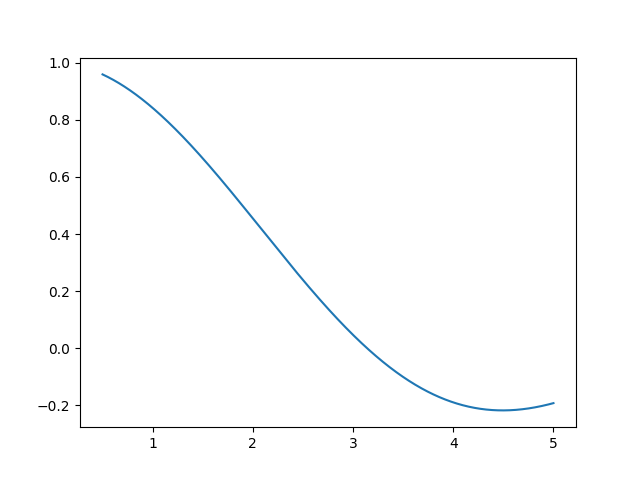
\includegraphics[scale=0.60]{images/Figure_2.png}
			\caption{$f(x)$ sur $[0.5~;\ 5]$}
		\end{figure}

\section{Algorithmes usuels}
	
	\subsection{Courbe d'une solution d'une équation différentielle} \label{corr:equa_diff} (Énoncé~: \ref{appl:equa_diff})
		
		On veut tracer une solution de cette équation différentielle~:
		\[
			\forall t \in [-1~;\ 10],\ (t^2 + 1)y' + (t - 1)^2y = t^3 - t^2 + t + 1
		\]
		Avec la condition initiale~: $y(-1) = 8$.
		
		En reprenant point par point~:
		\begin{enumerate}
			\item Assez simplement, on isole $y'$~:
			\[ \begin{array}{rll}
				(t^2 + 1)y' + (t - 1)^2y & = & t^3 - t^2 + t + 1 \\
				(t^2 + 1)y' & = & t^3 - t^2 + t + 1 - (t - 1)^2y \\
				y' & = & \frac{1}{(t^2 + 1)} \cdot (t^3 - t^2 + t + 1 - (t - 1)^2y)
			\end{array} \]
			Ainsi, on pose $\forall t \in [-1~;\ 10],\ y' = f(t, y) = \frac{1}{(t^2 + 1)} \cdot (t^3 - t^2 + t + 1 - (t - 1)^2y)$
			\begin{pythoncode}
				def f(t, y):
					return (1 / (t**2 + 1)) * (t**3 - t**2 + t + 1 - (t - 1)**2 * y)
			\end{pythoncode}
			
			\item On se place sur l'intervalle $[-1~;\ 10]$ avec un nombre arbitraire de points, on peut prendre $N = 1000$. Ainsi,
			\begin{pythoncode}
				h = (10 + 1) / 1000
				X = [-1 + n * h for n in range(1000)]
			\end{pythoncode}
			
			\item On initialise les ordonnées avec la condition initiale et on complète la liste~:
			\begin{pythoncode}
				Y = [8]
				for i in range(1000 - 1):
					Y.append(Y[i] + h * f(X[i], Y[i]))
			\end{pythoncode}
			
			\item Il ne reste plus qu'à tracer et à afficher~:
			\begin{pythoncode}
				plt.plot(X, Y)
				plt.show()
			\end{pythoncode}
		\end{enumerate}
	
	En résumé, le code complet~:
	\begin{pythoncode}
		import matplotlib.pyplot as plt
		
		def f(t, y):
			return (1 / (t**2 + 1)) * (t**3 - t**2 + t + 1 - (t - 1)**2 * y)
		
		h = (10 + 1) / 1000
		X = [-1 + n * h for n in range(1000)]
		
		Y = [8]
		for i in range(1000 - 1):
			Y.append(Y[i] + h * f(X[i], Y[i]))
		
		plt.plot(X, Y)
		plt.show()
	\end{pythoncode}
	
	La figure de gauche représente la solution de condition initiale $y(-1) = 8$ sur l'intervalle $[-1~;\ 10]$ et la figure de droite représente les solutions approchées pour des valeurs initiales entre $0$ et $8$ et $t$ entre $-1$ et $3$.
	
	\begin{tabular}{cc}
		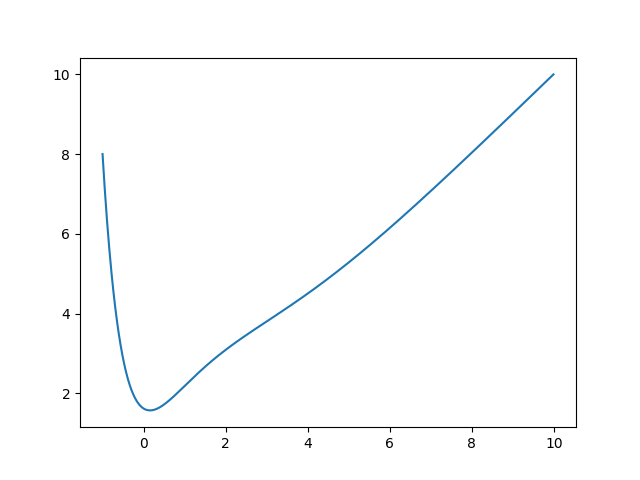
\includegraphics[scale=0.50]{images/Figure_5.png} &
		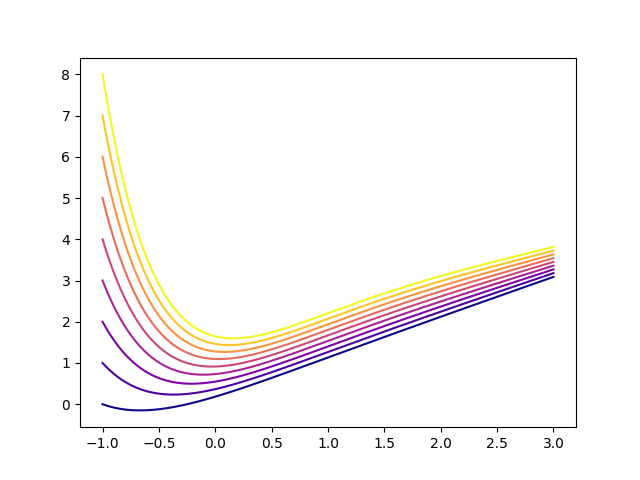
\includegraphics[scale=0.50]{images/Figure_6.png} \\
	\end{tabular}

\section{Programmation orientée objet}

	\subsection{Vecteurs} \label{corr:vecteurs} (Énoncé~: \ref{appl:vecteurs})
		
		\subsubsection{Initialisze l'objet}
		Le plus simple pour représenter un vecteur est d'utiliser une liste Python contenant les composantes du vecteurs selon les différentes coordonnées. Ainsi l'initialisation du vecteur va ressembler à~:
		\begin{pythoncode}
			class Vecteur:
				def __init__(self, composantes):
					self.composantes = composantes
					self.taille = len(composantes) # on stocke aussi la dimension du vecteur
		\end{pythoncode}
		
		\subsubsection{Afficher l'objet}
		Commencer par programmer l'affichage du nouvel objet permet de faire des tests assez rapidement ce qui est agréable. Ici rien de très compliqué.
		
		On pourrait transtyper deux fois notre liste de coordonnées~: une première fois pour avoir un tuple et une seconde fois pour avoir une chaîne de caractères. Cette solution fonctionne, mais n'est pas très élégante. Il est préférable de construire directement la représentation de l'objet~:
		\begin{pythoncode}
			def __repr__(self):
				composantes_str = [str(i) for i in self.composantes] # on construit la liste des composantes sous forme de chaînes de caractères
				return "(" + ", ".join(composantes_str) + ")"
		\end{pythoncode}
		
		\subsubsection{Addition de deux vecteurs}
		L'addition sur les vecteurs est une addition terme à terme, donc rien de très compliqué~:
		\begin{pythoncode}
			def __add__(self, vecteur):
				if self.taille != vecteur.taille:
					raise ValueError("on ne peut pas sommer deux vecteurs de tailles différentes") # On arrête l'exécution du programme et on renvoie une erreur de valeur
				
				resultat = [] # les composantes du nouveau vecteur
				for i in range(self.taille):
					resultat.append(self.composantes[i] + vecteur.composantes[i])
				
				return Vecteur(resultat) # on renvoie une instance de la classe Vecteur
		\end{pythoncode}
		
		\subsubsection{Multiplication par un scalaire}
		La multiplication entre un vecteur et un scalaire est simple~: chaque composante du vecteur est multipliée par le scalaire.
		\begin{pythoncode}
			def __mul__(self, scalaire):
				if not isinstance(scalaire, (int, float)):
					raise TypeError("ce n'est pas un scalaire") # si 'sclaire' n'est ni un int, ni un float, on arrête l'exécution du programme et on renvoie une erreur de type
				
				resultat = []
				for i in range(self.taille):
					resultat.append(scalaire * self.composantes[i])
				
				return Vecteur(resultat)
		\end{pythoncode}
		
		\subsubsection{Résumé et idées pour aller plus loin}
		Le code complet du vecteur est donc~:
		\begin{pythoncode}
			class Vecteur:
				def __init__(self, composantes):
					self.composantes = composantes
					self.taille = len(composantes)
					
				def __repr__(self):
					composantes_str = [str(i) for i in self.composantes]
					return "(" + ", ".join(composantes_str) + ")"
								
				__str__ = __repr__
				
				def __add__(self, vecteur):
					if self.taille != vecteur.taille:
						raise ValueError("on ne peut pas sommer deux vecteurs de tailles différentes")
					
					resultat = []
					for i in range(self.taille):
						resultat.append(self.composantes[i] + vecteur.composantes[i])
					
					return Vecteur(resultat)
				
				__radd__ = __add__
					
				def __mul__(self, scalaire):
					if not isinstance(scalaire, (int, float)):
						raise TypeError("ce n'est pas un scalaire")
					
					resultat = []
					for i in range(self.taille):
						resultat.append(scalaire * self.composantes[i])
					
					return Vecteur(resultat)
				
				__rmul__ = __mul__
		\end{pythoncode}
		
		Bien sûr il existe d'autres manipulations sur les vecteurs~: produit scalaire, norme, produit vectoriel etc. Ces fonctions ne sont pas expliquées ici, mais sont tout à fait faisables.
	
	\subsection{Polynômes} \label{corr:polynomes} (Énoncé~: \ref{appl:polynomes})
		
		\subsubsection{Initialiser l'objet}
		Avant d'écrire les méthodes, il faut penser à la manière dont l'objet va être représenté dans la classe. Ici, un polynôme est entièrement caractérisé par la donnée de ses coefficients, ainsi le polynôme va devoir avoir un attribut \python|coefficients| qui sera une liste. Le premier élément de la liste correspondra au coefficient de puissance nulle (indice 0 dans la liste), le second élément (indice 1) sera le coefficient de degré 1 etc.
		
		On impose par ailleurs un attribut \python|deg| qui correspond au degré du polynôme. Le degré correspond à la puissance maximale, de coefficient non nul. En supposant que la liste ne finit pas par un $0$, il s'agit de la longueur de la liste moins un.
		
		Avec les deux derniers paragraphes, on peut déjà rédiger la méthode \python|__init__|~:
		\begin{pythoncode}
			class Polynome:
				def __init__(self, coefficients):
					self.coefficients = coefficients
					self.deg = len(coefficients) - 1
		\end{pythoncode}
		
		\subsubsection{Afficher un polynôme}
		L'affichage maintenant. La liste des coefficients est triée par ordre croissant de puissance, donc le polynôme va être affiché dans cet ordre (on aurait pu l'afficher dans l'autre sens, mais cela ne présente pas beaucoup d'intérêt ici). L'idée va être de décomposer le polynôme en une liste de chaîne de caractères où chaque élément est un monôme qui compose le polynôme.
		
		Nous allons donc reccourir à une liste \python|monomes|. Ensuite, il va falloir faire une boucle \python|for| qui balaye les coeffiicents du polynôme à afficher en distinguant les cas~:
		\begin{itemize}
			\item si le coefficient vaut $0$, il n'y a rien à afficher
			\item si la puissance vaut $0$, $X^0 = 1$
			\item si la puissance vaut $1$, il suffit d'afficher \python|X| et non \python|X^1|
			\item sinon, on affiche sous la forme \python|coefficient X^puissance|
		\end{itemize}
		On ajoute ensuite le monôme à la liste. Et enfin on utilise \python|join| pour intercaler un signe \python|+| entre chaque monôme. Ainsi~:
		\begin{pythoncode}
			def __repr__(self):
		    monomes = []
		    for puissance in range(self.nb_coeff):
		        if self.coefficients[puissance] != 0:
		            if puissance == 0:
		                monomes.append(str(self.coefficients[puissance]))
		            elif puissance == 1:
		                monomes.append(str(self.coefficients[puissance]) + "X")
		            else:
		                monomes.append(str(self.coefficients[puissance]) + "X^" + str(puissance))
		    return " + ".join(monomes)
		\end{pythoncode}
		
		On peut également écrire~: \python|__str__ = __repr__| pour pouvoir transtyper le polynôme vers une chaîne de caractères.
		
		\subsubsection{Addition et soustraction de polynômes}
		L'addition et la soustraction se ressemblent beaucoup. Le degré du résultat est égal au maximum des degrés. Dans les deux cas, l'idée est de construire une liste \python|nouveaux_coeff| qui va contenir les coefficients du résultat et à la fin, on renvoie le polynôme associé à ces coefficients. Il y a trois cas à distinguer~:
		\begin{itemize}
			\item Si P n'a pas de coefficient de degré $i$, la somme est donc égale au coefficient de degré $i$ de Q.
			\item De manière symétrique, si Q n'a pas de coefficient de degré $i$, la somme est alors égale au coefficient de degré $i$ de P.
			\item Sinon, il s'agit de la somme des coefficients.
		\end{itemize}
		On obtient alors la code~:
		\begin{pythoncode}
			def __add__(self, P):
				nouveaux_coeff = []
				for i in range(max(self.deg, P.deg) + 1):
				    if self.deg < i:
				        nouveaux_coeff.append(P.coefficients[i])
				    elif P.deg < i:
				        nouveaux_coeff.append(self.coefficients[i])
				    else:
				        nouveaux_coeff.append(self.coefficients[i] + P.coefficients[i])
				return Polynome(nouveaux_coeff)
		\end{pythoncode}
		
		On procède de même avec la soustraction.
		
		\subsubsection{Évaluation du polynôme en une valeur}
		Il s'agit d'une méthode à part, assez simple. Il suffit de "remplacer" le $X$ du polynôme par la valeur donnée. Nous allons commencer par définir une variable \python|resultat|, initialisée à $0$ au début. On va ensuite balayer la liste des coefficients du polynômes. Par construction, l'indice du coefficient correspond à la puissance du monôme, ainsi~:
		\begin{pythoncode}
			def __call__(self, X):
				resultat = 0
				for puissance in range(self.deg + 1):
				    resultat += self.coefficients[puissance] * X ** puissance

				return resultat
		\end{pythoncode}
		
		\subsubsection{Dérivation d'un polynôme}
			En appliquant la formule explicite pour la dérivation~:
			\begin{pythoncode}
				def derivee(self):
					nouveaux_coeff = [0]
					for puissance in range(self.deg + 1):
						if puissance:
						    nouveaux_coeff[puissance - 1] = self.coefficients[puissance] * puissance
						    nouveaux_coeff.append(0)
					return Polynome(nouveaux_coeff)
			\end{pythoncode}
		
		\subsubsection{Code complet}
		\begin{pythoncode}
			class Polynome:
				def __init__(self, coefficients):
					self.coefficients = coefficients

					self.deg = len(coefficients) - 1

				def __repr__(self):
					monomes = []
					for puissance in range(self.deg + 1):
						if self.coefficients[puissance] != 0:
						    if puissance == 0:
						        monomes.append(str(self.coefficients[puissance]))
						    elif puissance == 1:
						        monomes.append(str(self.coefficients[puissance]) + "X")
						    else:
						        monomes.append(str(self.coefficients[puissance]) + "X^" + str(puissance))
					return " + ".join(monomes)

				__str__ = __repr__

				def __add__(self, P):
					nouveaux_coeff = []
					for i in range(max(self.deg, P.deg) + 1):
						if self.deg < i:
						    nouveaux_coeff.append(P.coefficients[i])
						elif P.deg < i:
						    nouveaux_coeff.append(self.coefficients[i])
						else:
						    nouveaux_coeff.append(self.coefficients[i] + P.coefficients[i])
					return Polynome(nouveaux_coeff)

				def __sub__(self, P):
					nouveaux_coeff = []
					for i in range(max(self.deg, P.deg) + 1):
						if self.deg < i:
						    nouveaux_coeff.append(-P.coefficients[i])
						elif P.deg < i:
						    nouveaux_coeff.append(self.coefficients[i])
						else:
						    nouveaux_coeff.append(self.coefficients[i] - P.coefficients[i])
					return Polynome(nouveaux_coeff)

				def __call__(self, X):
					resultat = 0
					for puissance in range(self.deg + 1):
						resultat += self.coefficients[puissance] * X ** puissance

					return resultat

				def derivee(self):
					nouveaux_coeff = [0]
					for puissance in range(self.deg + 1):
						if puissance:
						    nouveaux_coeff[puissance - 1] = self.coefficients[puissance] * puissance
						    nouveaux_coeff.append(0)
					return Polynome(nouveaux_coeff)
		\end{pythoncode}
		
		
		
	

\end{document}
